% Options for packages loaded elsewhere
\PassOptionsToPackage{unicode}{hyperref}
\PassOptionsToPackage{hyphens}{url}
%
\documentclass[
  ignorenonframetext,
]{beamer}
\usepackage{pgfpages}
\setbeamertemplate{caption}[numbered]
\setbeamertemplate{caption label separator}{: }
\setbeamercolor{caption name}{fg=normal text.fg}
\beamertemplatenavigationsymbolsempty
% Prevent slide breaks in the middle of a paragraph
\widowpenalties 1 10000
\raggedbottom
\setbeamertemplate{part page}{
  \centering
  \begin{beamercolorbox}[sep=16pt,center]{part title}
    \usebeamerfont{part title}\insertpart\par
  \end{beamercolorbox}
}
\setbeamertemplate{section page}{
  \centering
  \begin{beamercolorbox}[sep=12pt,center]{part title}
    \usebeamerfont{section title}\insertsection\par
  \end{beamercolorbox}
}
\setbeamertemplate{subsection page}{
  \centering
  \begin{beamercolorbox}[sep=8pt,center]{part title}
    \usebeamerfont{subsection title}\insertsubsection\par
  \end{beamercolorbox}
}
\AtBeginPart{
  \frame{\partpage}
}
\AtBeginSection{
  \ifbibliography
  \else
    \frame{\sectionpage}
  \fi
}
\AtBeginSubsection{
  \frame{\subsectionpage}
}
\usepackage{amsmath,amssymb}
\usepackage{iftex}
\ifPDFTeX
  \usepackage[T1]{fontenc}
  \usepackage[utf8]{inputenc}
  \usepackage{textcomp} % provide euro and other symbols
\else % if luatex or xetex
  \usepackage{unicode-math} % this also loads fontspec
  \defaultfontfeatures{Scale=MatchLowercase}
  \defaultfontfeatures[\rmfamily]{Ligatures=TeX,Scale=1}
\fi
\usepackage{lmodern}
\usetheme[]{default}
\usefonttheme{professionalfonts}
\ifPDFTeX\else
  % xetex/luatex font selection
\fi
% Use upquote if available, for straight quotes in verbatim environments
\IfFileExists{upquote.sty}{\usepackage{upquote}}{}
\IfFileExists{microtype.sty}{% use microtype if available
  \usepackage[]{microtype}
  \UseMicrotypeSet[protrusion]{basicmath} % disable protrusion for tt fonts
}{}
\makeatletter
\@ifundefined{KOMAClassName}{% if non-KOMA class
  \IfFileExists{parskip.sty}{%
    \usepackage{parskip}
  }{% else
    \setlength{\parindent}{0pt}
    \setlength{\parskip}{6pt plus 2pt minus 1pt}}
}{% if KOMA class
  \KOMAoptions{parskip=half}}
\makeatother
\usepackage{xcolor}
\newif\ifbibliography
\usepackage{graphicx}
\makeatletter
\def\maxwidth{\ifdim\Gin@nat@width>\linewidth\linewidth\else\Gin@nat@width\fi}
\def\maxheight{\ifdim\Gin@nat@height>\textheight\textheight\else\Gin@nat@height\fi}
\makeatother
% Scale images if necessary, so that they will not overflow the page
% margins by default, and it is still possible to overwrite the defaults
% using explicit options in \includegraphics[width, height, ...]{}
\setkeys{Gin}{width=\maxwidth,height=\maxheight,keepaspectratio}
% Set default figure placement to htbp
\makeatletter
\def\fps@figure{htbp}
\makeatother
\setlength{\emergencystretch}{3em} % prevent overfull lines
\providecommand{\tightlist}{%
  \setlength{\itemsep}{0pt}\setlength{\parskip}{0pt}}
\setcounter{secnumdepth}{-\maxdimen} % remove section numbering
\usepackage{fancyhdr}
\usepackage{lastpage}
\setbeamertemplate{navigation symbols}{}
\setbeamertemplate{footline}[page number]
\pagenumbering{arabic}
% \usepackage[mathbf,mathcal]{euler}

\ifLuaTeX
  \usepackage{selnolig}  % disable illegal ligatures
\fi
\IfFileExists{bookmark.sty}{\usepackage{bookmark}}{\usepackage{hyperref}}
\IfFileExists{xurl.sty}{\usepackage{xurl}}{} % add URL line breaks if available
\urlstyle{same}
\hypersetup{
  hidelinks,
  pdfcreator={LaTeX via pandoc}}

\title{Tipos de Experimentos en Ciencias Sociales}
\author{Luciana Cantera y Lucía Suarez\\
Diseño e implementación de experimentos en ciencias sociales\\
\emph{Departamento de Economía (UdelaR)}}
\date{}

\begin{document}
\frame{\titlepage}

\begin{frame}{Tema 6. Tipos de experimentos en ciencias sociales}
\protect\hypertarget{tema-6.-tipos-de-experimentos-en-ciencias-sociales}{}
\begin{enumerate}
\tightlist
\item
  Experimentos de Campo
\item
  Experimentos Naturales
\item
  Experimentos de Encuesta
\item
  Experimentos de Laboratorio
\end{enumerate}
\end{frame}

\hypertarget{experimentos-de-campo}{%
\section{Experimentos de Campo}\label{experimentos-de-campo}}

\begin{frame}{Lecturas}
\protect\hypertarget{lecturas}{}
\begin{itemize}
\item
  Gerber, Alan S, and Donald P Green. 2012. Field Experiments: Design,
  Analysis, and Interpretation. WW Norton.
\item
  List, J. A. (2011). ``Why economists should conduct field experiments
  and 14 tips for pulling one off''. The Journal of Economic
  Perspectives, 25(3):3--15
\end{itemize}
\end{frame}

\begin{frame}{¿Qué son los experimentos de campo?}
\protect\hypertarget{quuxe9-son-los-experimentos-de-campo}{}
\begin{itemize}
\tightlist
\item
  Estudios aleatorizados que se llevan a cabo en entornos reales
\item
  Campo: evoca a los primeros experimentos agrícolas que se realizaban
  en los campos
\item
  Varios criterios a tener en cuenta:

  \begin{itemize}
  \tightlist
  \item
    El \textbf{tratamiento} utilizado en el estudio se parece a la
    \emph{intervención de interés} en el mundo
  \item
    Los \textbf{participantes} se parencen a los \emph{actores que
    normalmente se encuentran con estas intervenciones}
  \item
    El \textbf{contexto} en el que los sujetos perciben el tratamiento
    se parece al \emph{contexto de interes}
  \item
    Las medidas de los \textbf{resultados} se parecen a los
    \emph{resultados reales de interés} teórico y práctico
  \end{itemize}
\end{itemize}
\end{frame}

\begin{frame}{¿Qué son los experimentos de campo?}
\protect\hypertarget{quuxe9-son-los-experimentos-de-campo-1}{}
\begin{itemize}
\item
  Experimentos que intentan ser lo más realistas y discretos posibles
  para probar hipótesis más específicas del contexto
\item
  Estudios experimentales con poco contenido de campo:

  \begin{itemize}
  \tightlist
  \item
    realizan intervenciones reales en entornos artificiales a sujetos
    que son conscientes que forman parte de un estudio
  \end{itemize}
\end{itemize}
\end{frame}

\begin{frame}{Algunas ventajas de los experimentos de campo}
\protect\hypertarget{algunas-ventajas-de-los-experimentos-de-campo}{}
\begin{itemize}
\tightlist
\item
  Resuelve algunas amenzas a la inferencia cuando se extraen
  generalizaciones a partir de resultados obtenidos en entornos de
  laboratorio
\item
  Se diseñan para que las generalizaciones dependan menos de las
  suposiciones
\item
  La intervención suele ser discreta:

  \begin{itemize}
  \tightlist
  \item
    la intervención y la medición de los resultados no alerta a los
    sujetos del hecho de que están siendo estudiados
  \end{itemize}
\item
  Tienden a controlar el comportamiento durante largos períodos de
  tiempo

  \begin{itemize}
  \tightlist
  \item
    Fuertes efectos instantaneos que decaen con el tiempo
  \end{itemize}
\end{itemize}
\end{frame}

\begin{frame}{Algunas limitantes de los experimentos de campo}
\protect\hypertarget{algunas-limitantes-de-los-experimentos-de-campo}{}
\begin{itemize}
\tightlist
\item
  Si los sujetos saben que están siendo estudiados o si perciben que el
  tratamiento que han recibido debe provocar un determinado tipo de
  respuesta, es posible que expresen las opiniones o informen del
  comportamiento que creen que el experimentador quiere oír
\item
  No se pueden administrar tan fácilmente múltiples variaciones de un
  tratamiento para probar proposiciones teóricas precisas
\item
  A menudo resulta difícil ponerlos en práctica:

  \begin{itemize}
  \tightlist
  \item
    los investigadores no toman decisiones unilaterales
  \item
    coordinación entre investigadores y quienes proporcionan datos o
    llevan adelante la intervención
  \end{itemize}
\end{itemize}
\end{frame}

\begin{frame}{Evaluaciones de programas}
\protect\hypertarget{evaluaciones-de-programas}{}
Muchos experimentos de campo adoptan la forma de ``evaluaciones de
programas'' diseñadas para calibrar hasta qué punto los recursos se
despliegan con eficacia.

Ejemplo: para comprobar si la campaña de publicidad televisiva de una
candidata política aumenta su popularidad, un experimento de campo
podría aleatorizar las zonas geográficas en las que se despliegan los
anuncios y medir las diferencias de apoyo de los votantes.
\end{frame}

\begin{frame}{Ejemplo\footnote<.->{Borraz, F., Caro, A., Caño-Guiral, M.
  et al (2022) ``A randomised evaluation of a financial literacy
  programme for upper secondary school students in Uruguay.'' Int Rev
  Educ 68, 885--896.}}
\protect\hypertarget{ejemplo}{}
A randomised evaluation of a financial literacy programme for upper
secondary school students in Uruguay.


\includegraphics[width=0.7\textwidth,height=\textheight]{figs/Resumen_borraz_2022.png}
\end{frame}

\begin{frame}{Nudge\footnote<.->{Bloomfield, J., A. Balsa, A. Cid.
  (2022). ``Using Behavioral Insights in Early Childhood Interventions:
  the Effects of Crianza Positiva E-Messaging Program on Parental
  Investment.'' Review of Economics of the Household. 1-36.}}
\protect\hypertarget{nudge}{}
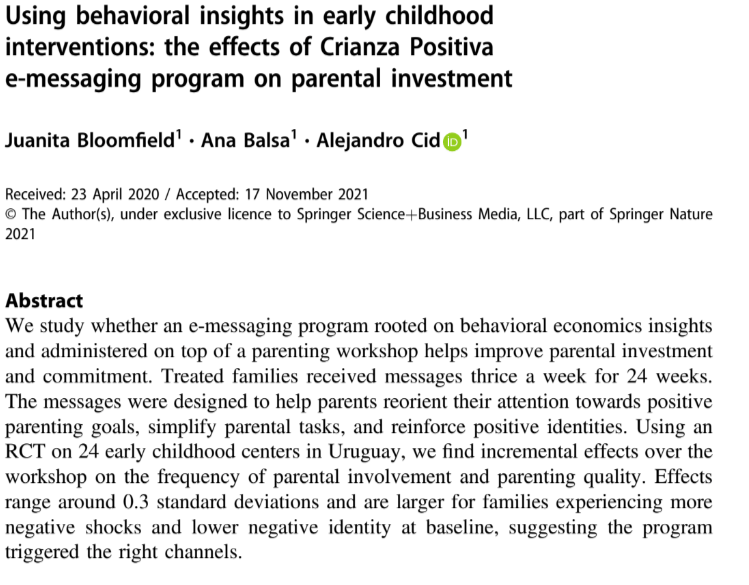
\includegraphics[width=0.8\textwidth,height=\textheight]{figs/Resumen_Balsa.png}
\end{frame}

\begin{frame}{Nudge\footnote<.->{\url{https://www.socialscienceregistry.org/trials/6321}}}
\protect\hypertarget{nudge-1}{}
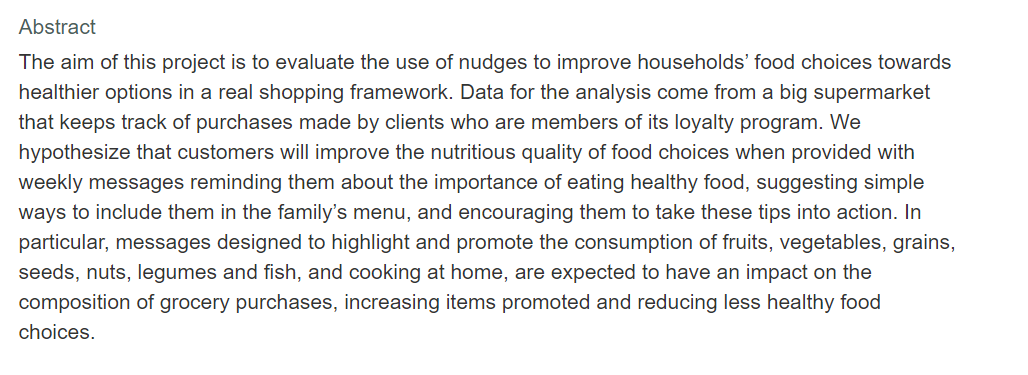
\includegraphics{figs/Resumen_Noboa.png}
\end{frame}

\begin{frame}{Generalización y validez externa}
\protect\hypertarget{generalizaciuxf3n-y-validez-externa}{}
\begin{itemize}
\tightlist
\item
  La aleatorización aporta un alto grado de validez interna al estudio
\item
  Pero los resultados obtenidos en un lugar y momento particular pueden
  no ser válidos en otros contextos (validez externa)
\item
  Este es un problema general, no solo de los experimentos
\end{itemize}

Una opción de solución:

La iniciativa Metaketa de EGAP: tomar una pregunta amplia, que tenga
relevancia de política para los gobiernos, identificando la intervención
que es pretendida e implementar un grupo de estudios coordinados que
puedan proveer respuestas confiables a la pregunta.
\end{frame}

\begin{frame}{Consideraciones éticas}
\protect\hypertarget{consideraciones-uxe9ticas}{}
\begin{itemize}
\tightlist
\item
  La investigación en ciencias sociales usualmente involucra a sujetos
  humanos, de quienes recogemos datos.
\item
  Por su naturaleza, la investigación experimental es intervencionista.
  Los experimentos de campo buscan generar impactos de la vida real en
  la sociedad, los procesos políticos y los resultados económicos.
\item
  Esto conlleva a responsabilidades éticas como investigadores.
\end{itemize}
\end{frame}

\begin{frame}{Consideraciones éticas}
\protect\hypertarget{consideraciones-uxe9ticas-1}{}
\begin{itemize}
\tightlist
\item
  Tener cuidado con los beneficios potenciales del conocimiento que se
  obtendrá frente a los riesgos potenciales de daño a las personas y
  comunidades donde realizamos la investigación.
\item
  Esto no es tan fácil:

  \begin{itemize}
  \tightlist
  \item
    El que un resultado sea bueno o malo puede depender de la
    perspectiva de cada uno, lo que a veces dificulta el equilibrio
    entre riesgos y beneficios.
  \item
    Somos propensos a sobrestimar significativamente los beneficios del
    conocimiento, por lo que debemos ser cautelosos y tener controles
    externos.
  \end{itemize}
\end{itemize}
\end{frame}

\hypertarget{experimentos-naturales}{%
\section{Experimentos Naturales}\label{experimentos-naturales}}

\begin{frame}{Lecturas}
\protect\hypertarget{lecturas-1}{}
\begin{itemize}
\item
  Dunning, Thad. 2012. Natural Experiments in the Social Sciences
  Natural Experiments in the Social Sciences.
\item
  Dunning, Thad. 2008. ``Improving Causal Inference: Strengths and
  Limitations of Natural Experiments.'' Political Research Quarterly
  61(2): 282--293.
\end{itemize}
\end{frame}

\begin{frame}{¿Qué son los Experimentos Naturales?}
\protect\hypertarget{quuxe9-son-los-experimentos-naturales}{}
\begin{itemize}
\tightlist
\item
  Los datos usados en experimentos naturales surgen de fenómenos
  ocurridos en la ``naturaleza''

  \begin{itemize}
  \tightlist
  \item
    Fenómenos relacionados a procesos sociales y políticos
  \end{itemize}
\item
  Como la asignación al tratamiento no es manipulada por el
  investigador, son estudios observacionales

  \begin{itemize}
  \tightlist
  \item
    Crean situaciones que se aproximan a los verdaderos experimentos
  \end{itemize}
\item
  Sin embargo, el investigador puede afirmar de forma creíble que la
  asignación es ``como si'' fuera aleatoria (as if random)
\end{itemize}
\end{frame}

\begin{frame}{El primer experimento natural estudiado (Snow)}
\protect\hypertarget{el-primer-experimento-natural-estudiado-snow}{}
\begin{columns}
\begin{column}{0.8\textwidth}
\begin{itemize}
\item En el siglo XIX Londres sufrió de una epidemia de cólera
\begin{itemize}
\item Había diversas teorías para explicar la transmisión
\item Snow sugería que la enfermedad se transmitía a través del agua
\end{itemize}
\item Londres era abastecido por dos grandes compañías de agua
\item Una de ellas trasladó su tubería de captación río arriba en el Támesis: "obtuvo un suministro de agua bastante libre de las aguas residuales de Londres"
\item Esto proporcionó un experimento natural
\item Las casas abastecidas por la empresa con el nuevo suministro, vieron reducidas las tasas de mortalidad por cólera
\end{itemize}
\end{column}
\begin{column}{0.2\textwidth}
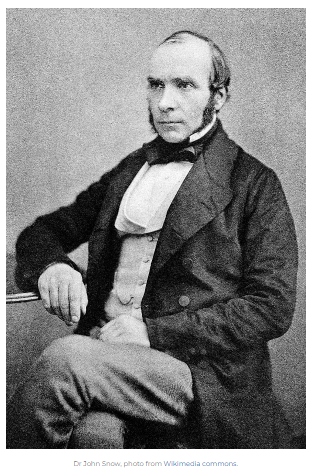
\includegraphics[width=\textwidth]{figs/john_snow.png}
\end{column}
\end{columns}
\end{frame}

\begin{frame}{¿Por qué el trabajo de Snow es creíble como experimento
natural?}
\protect\hypertarget{por-quuxe9-el-trabajo-de-snow-es-creuxedble-como-experimento-natural}{}
\begin{columns}
\begin{column}{0.6\textwidth}
\begin{itemize}
\item La asignación a las condiciones de tratamiento y control fue "as if random"
\item La provisión de agua es independiente de factores observables e inobservables que podrían influenciar las tasas de muerte por cólera
\item La gente no se movió en respuesta del tratamiento
\item Grupos de tratamiento y control eran balanceados en relación a otras variables medibles que podrían explicar las tasas de muerte por cólera
\end{itemize}
\end{column}
\begin{column}{0.4\textwidth}
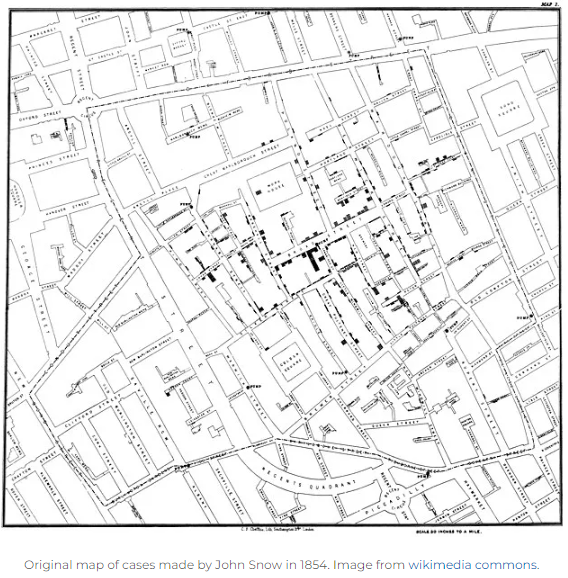
\includegraphics[width=\textwidth]{figs/map_snow.png}
\end{column}
\end{columns}
\end{frame}

\begin{frame}{¿Por qué usar Experimentos Naturales?}
\protect\hypertarget{por-quuxe9-usar-experimentos-naturales}{}
\begin{itemize}
\tightlist
\item
  Hay contextos donde realizar experimentos directos es caro, tiene
  problemas éticos, o impráctico
\item
  Muchas de las causas que más importan a los investigadores no son
  manipulables
\item
  En estos casos los experimentos naturales proporcionan una herramienta
  valiosa
\end{itemize}
\end{frame}

\begin{frame}{Descubriendo Experimentos Naturales}
\protect\hypertarget{descubriendo-experimentos-naturales}{}
\begin{itemize}
\tightlist
\item
  \textit{Standard}

  \begin{itemize}
  \tightlist
  \item
    Utilizar un dispositivo aleatorio real con una distribución de
    probabilidades conocida que asigna a los sujetos a la condición de
    tratamiento y control (ej. lotería)
  \item
    Aprovechar la existencia de fronteras políticas o jurisdiccionales
    que separen poblaciones similares de individuos, comunidades,
    empresas u otras unidades de análisis
  \item
    Fenómenos naturales como clima
  \end{itemize}
\item
  Diseño en Regresión Discontinua (RDD)

  \begin{itemize}
  \tightlist
  \item
    Reglas institucionales que crean umbrales estrictos que asignan
    sujetos a control y tratamiento
  \item
    Es clave que los individuos no se auto-seleccionen en tratamiento
  \end{itemize}
\item
  Diseños de Variables Instrumentales
\end{itemize}
\end{frame}

\begin{frame}{Experimentos Naturales \textit{Standard} comunes}
\protect\hypertarget{experimentos-naturales-comunes}{}
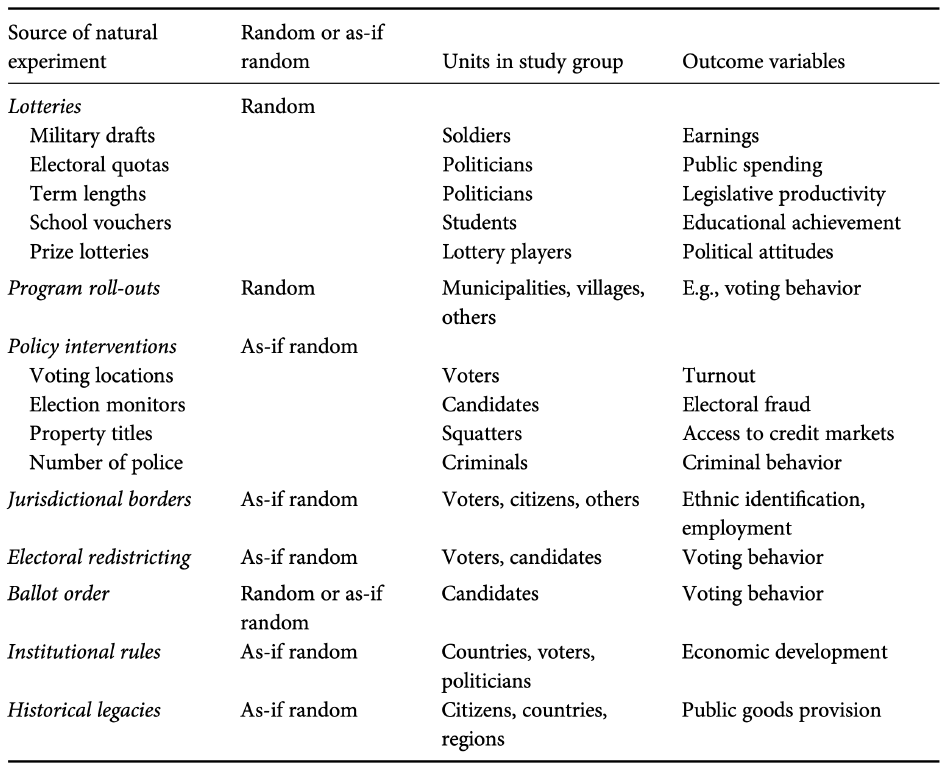
\includegraphics{figs/nat_exp_standard1.png}
\end{frame}

\begin{frame}{Experimentos Naturales \textit{Standard} con as-if
randomization}
\protect\hypertarget{experimentos-naturales-con-as-if-randomization}{}
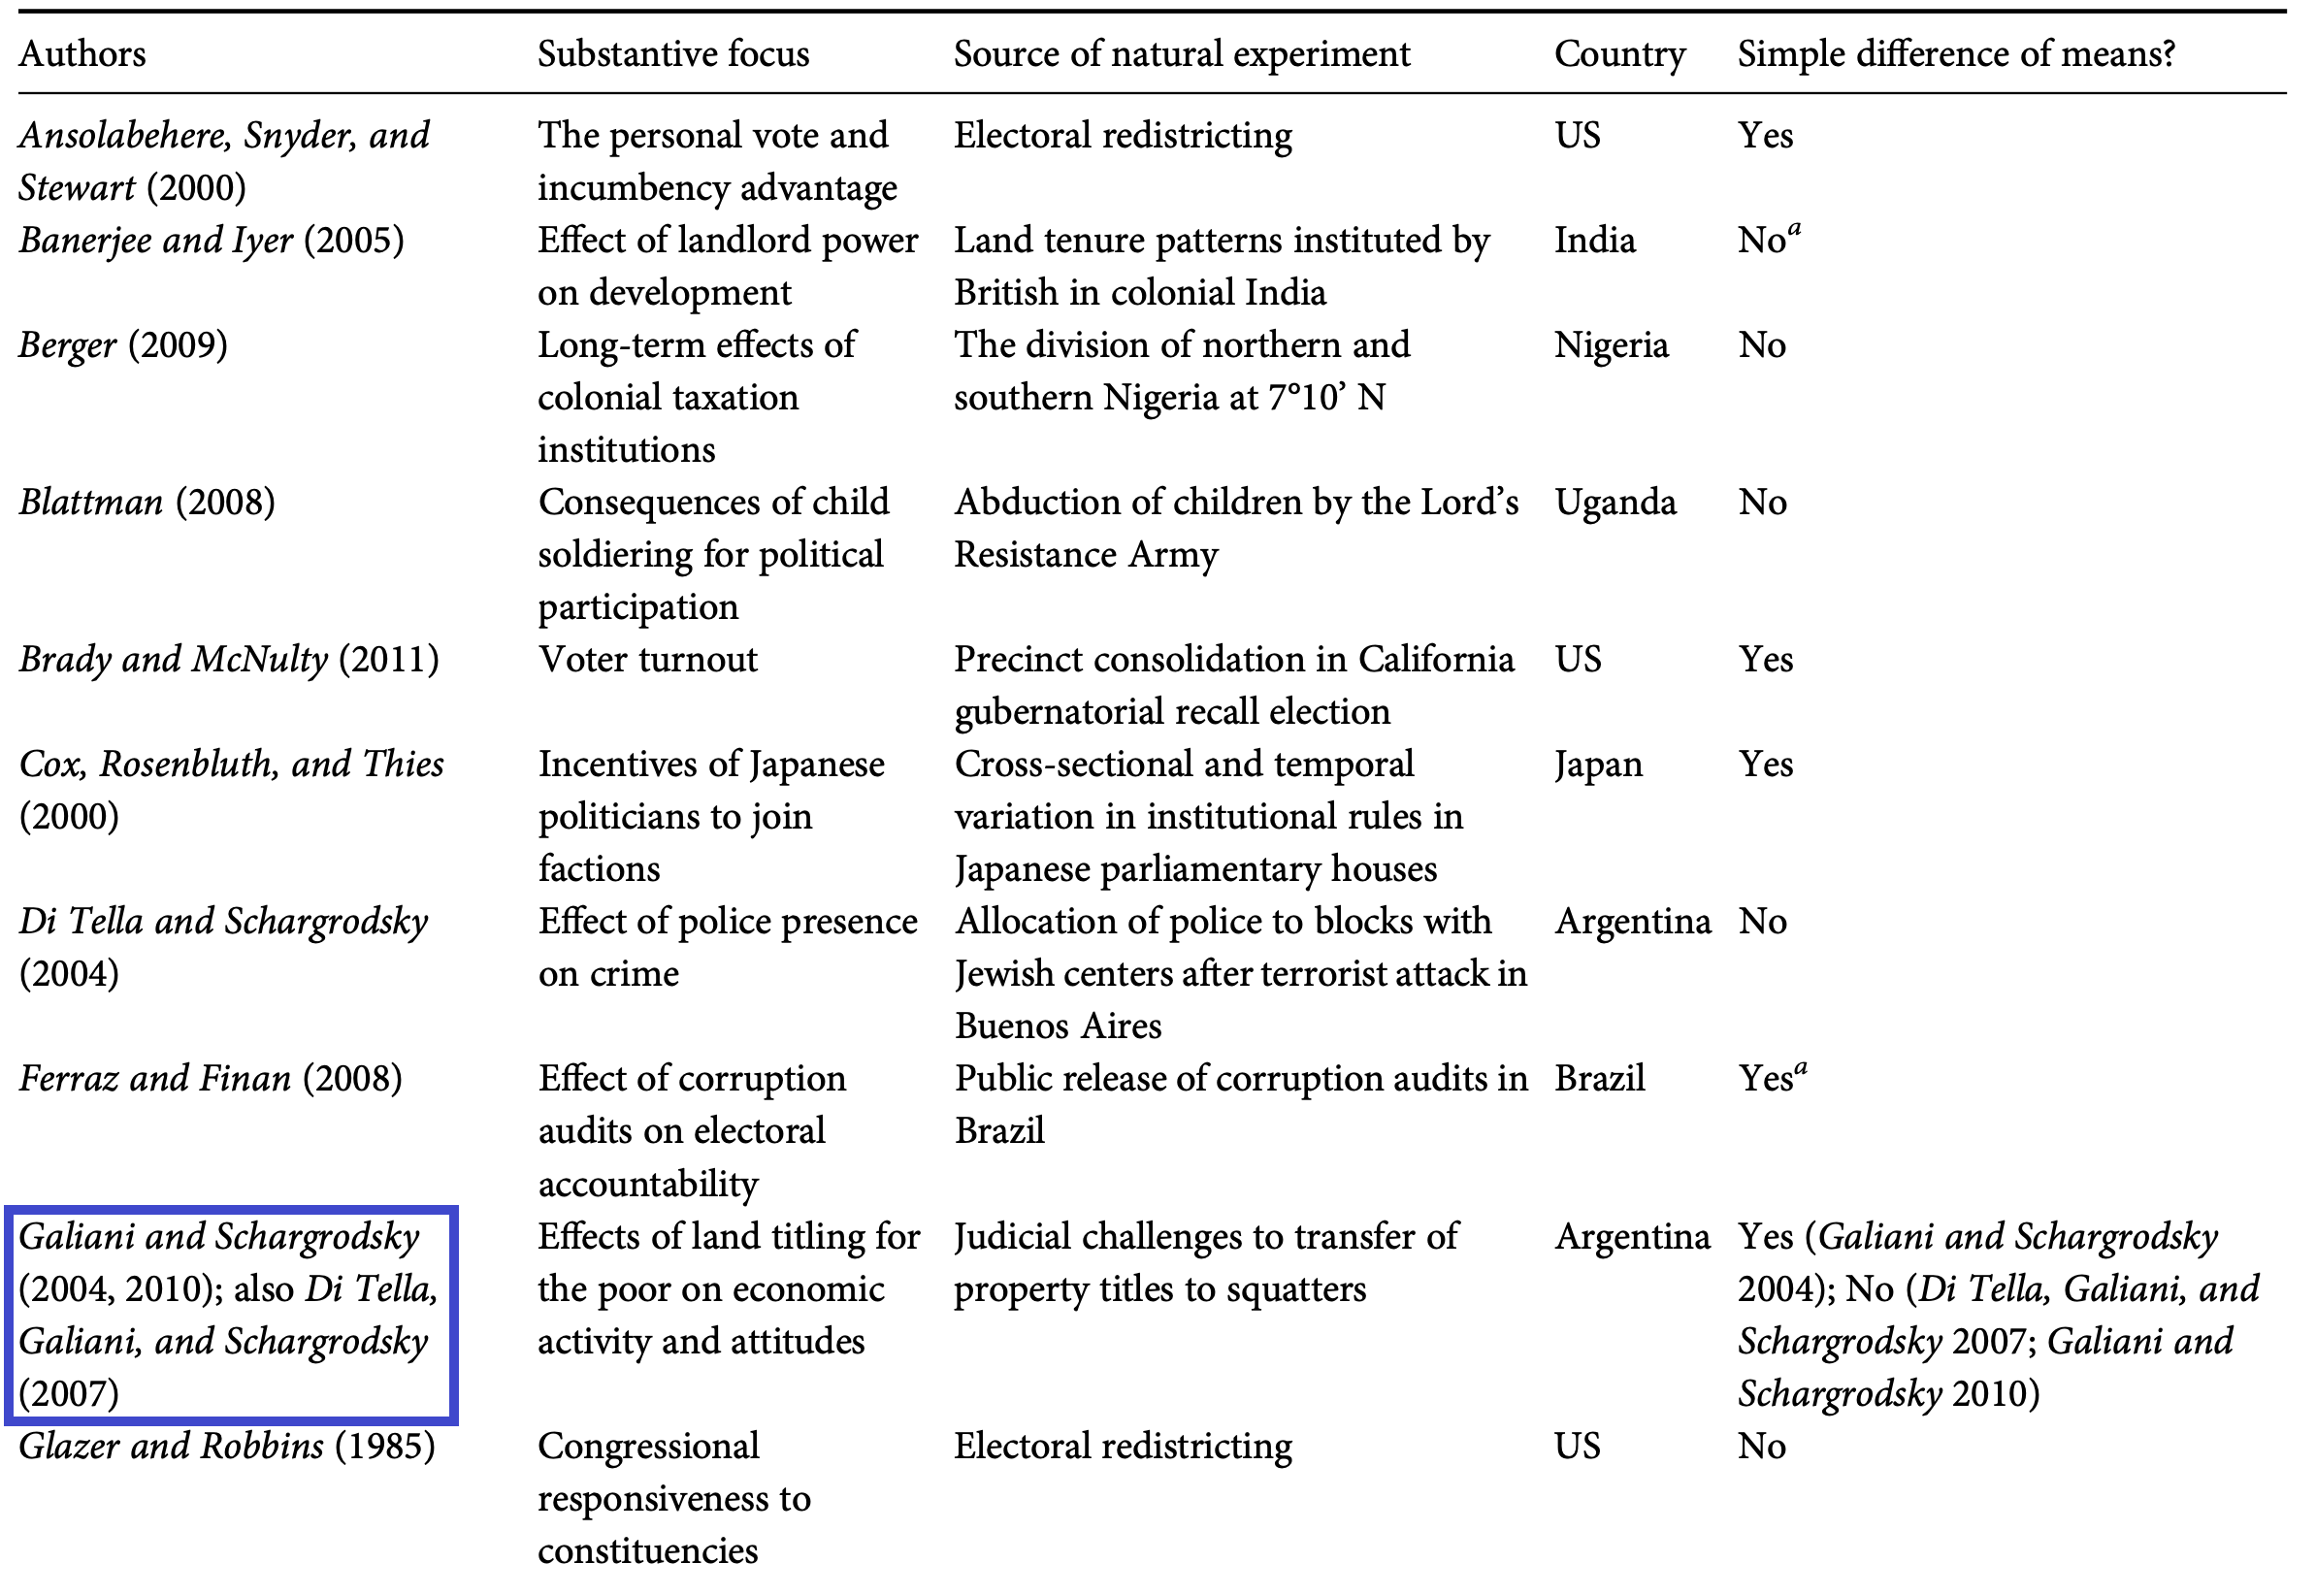
\includegraphics{figs/nat_exp_standard2.png}
\end{frame}

\begin{frame}{Experimentos Naturales \textit{Standard} con as-if
randomization}
\protect\hypertarget{experimentos-naturales-con-as-if-randomization-1}{}
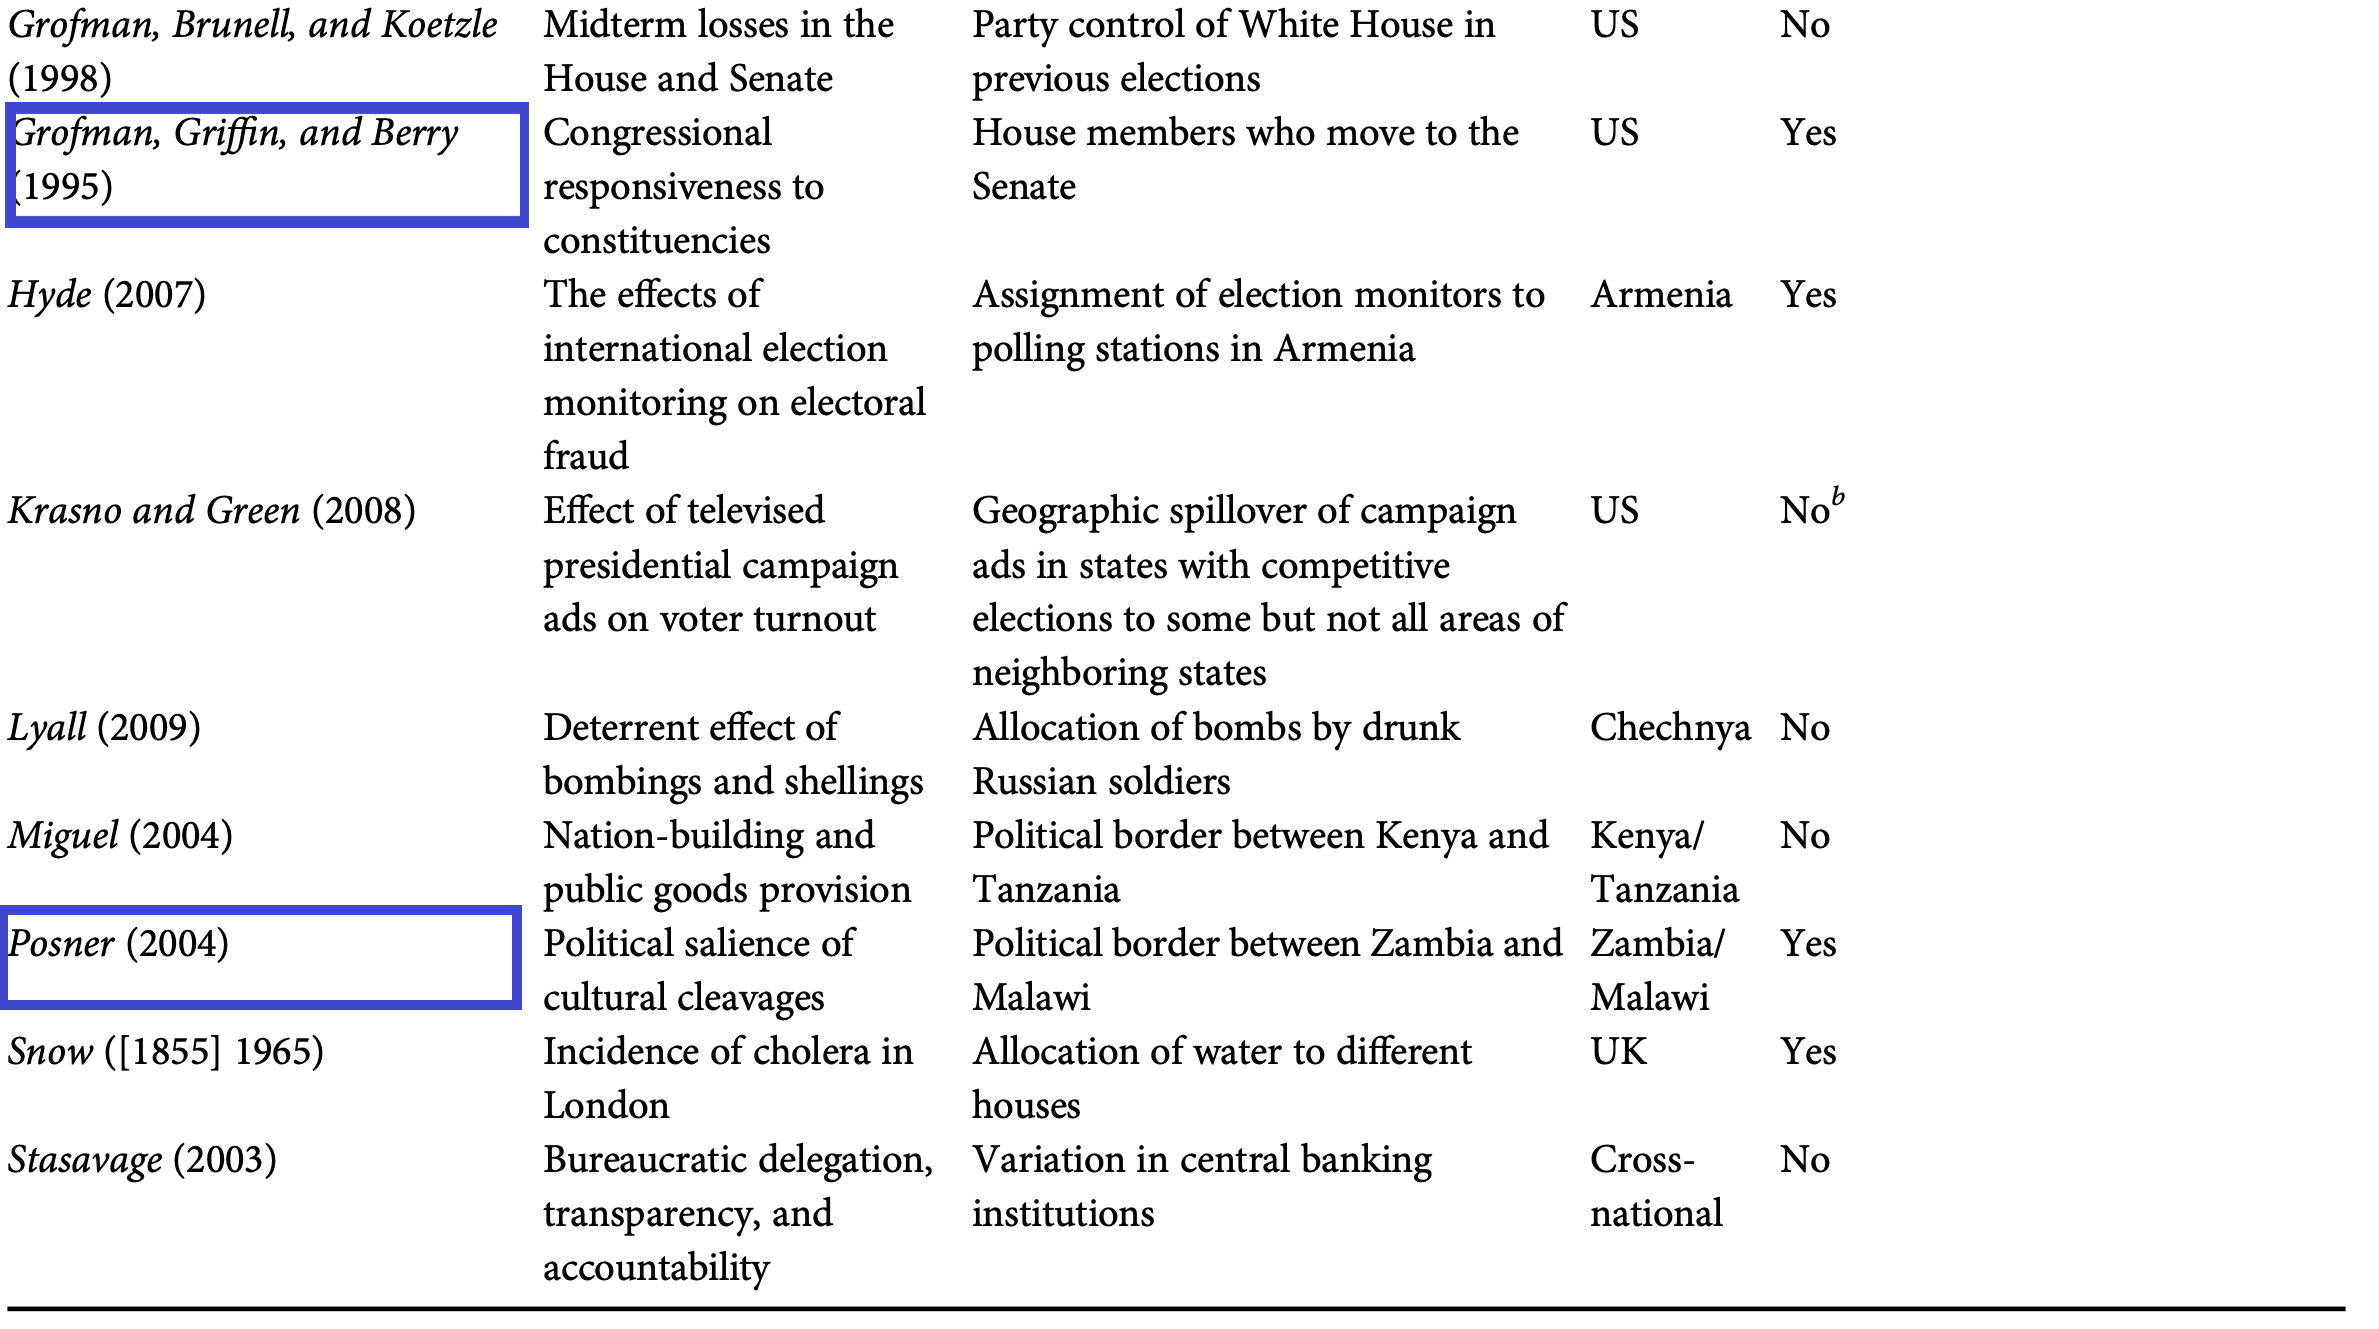
\includegraphics{figs/nat_exp_standard3.png}
\end{frame}

\begin{frame}{Diseños en Regresión Discontinua: fuentes seleccionadas}
\protect\hypertarget{diseuxf1os-en-regresiuxf3n-discontinua-fuentes-seleccionadas}{}
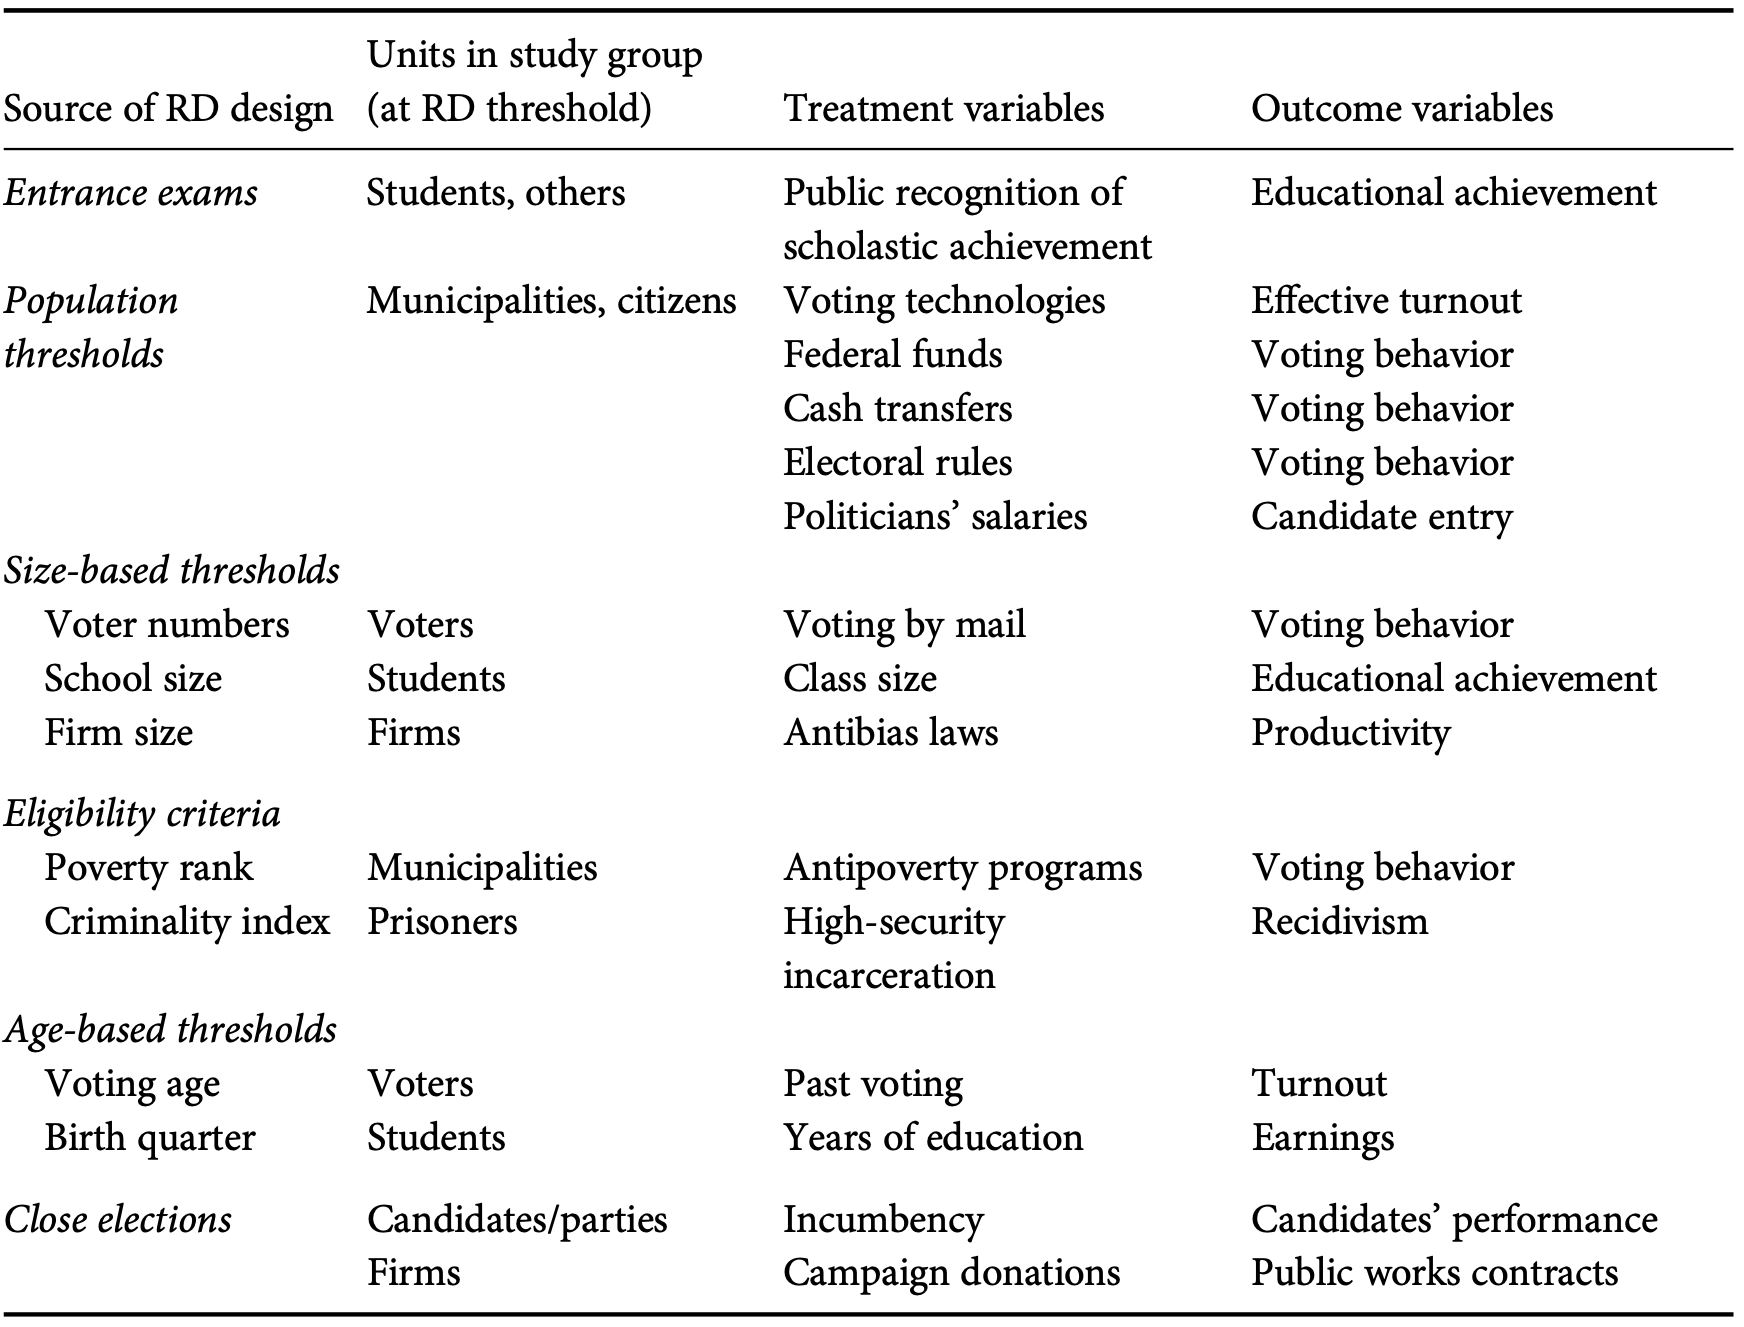
\includegraphics{figs/nat_exp_RDD1.png}
\end{frame}

\begin{frame}{Diseños en Regresión Discontinua: Ejemplos}
\protect\hypertarget{diseuxf1os-en-regresiuxf3n-discontinua-ejemplos}{}
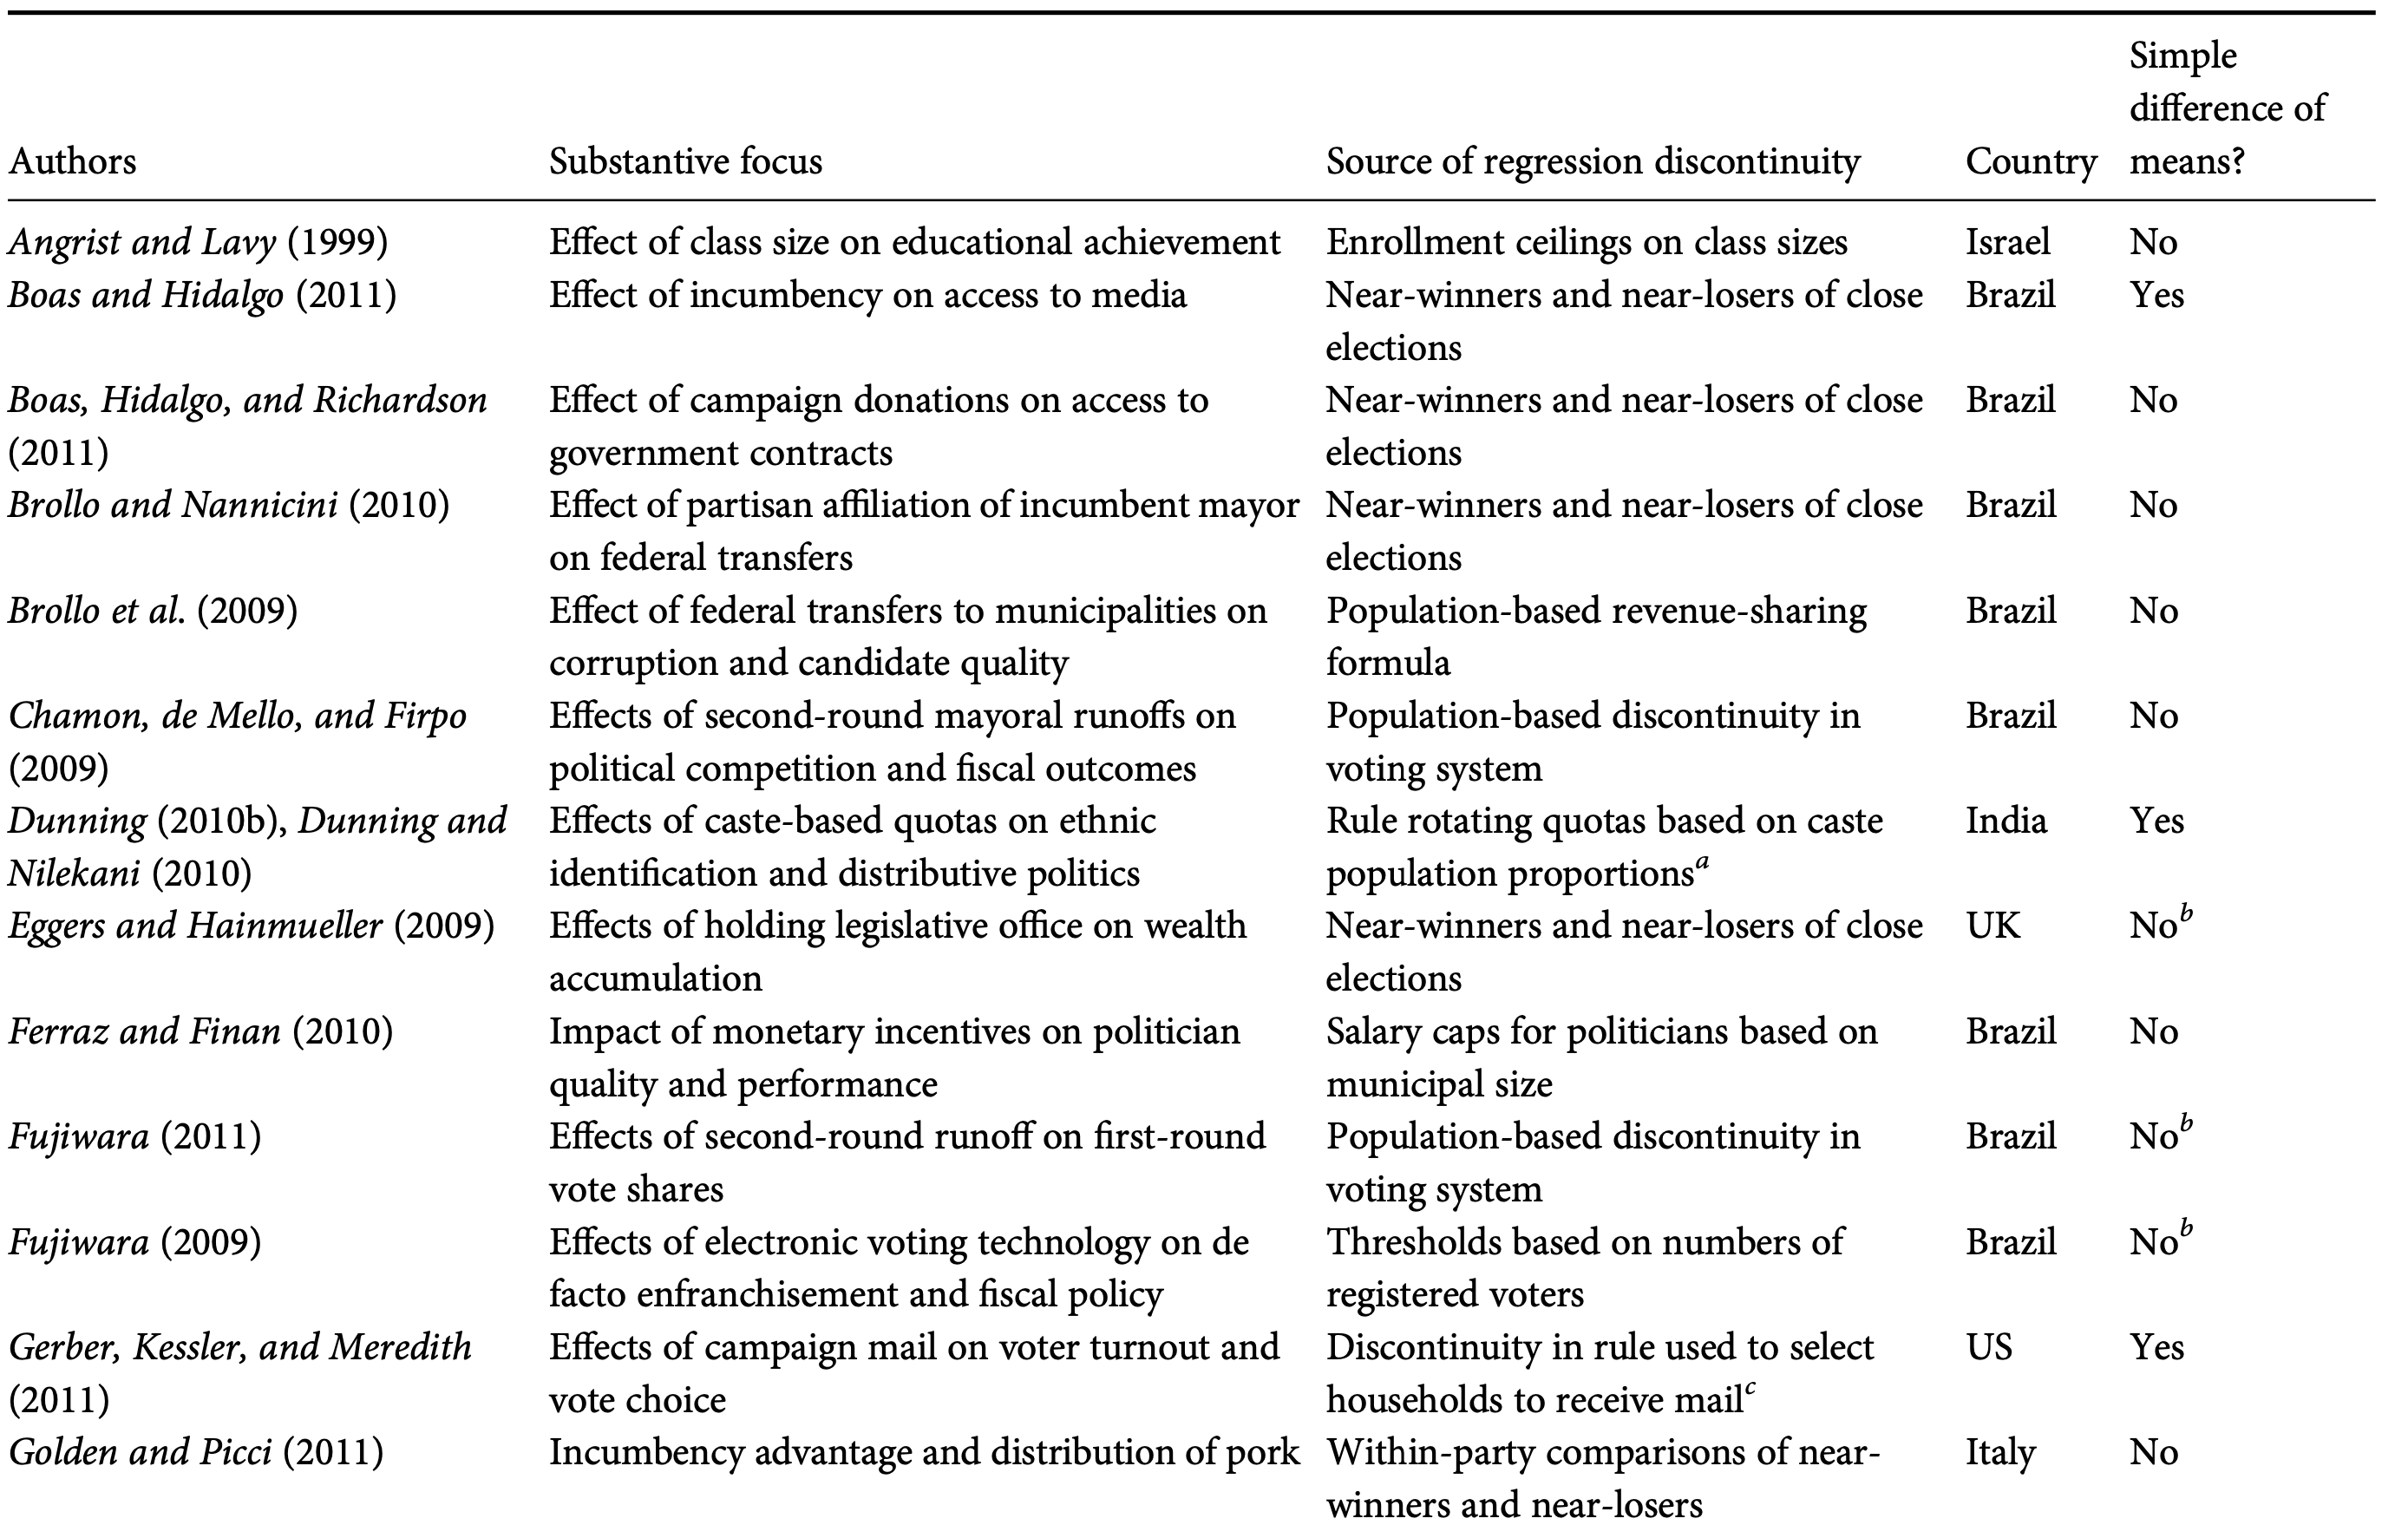
\includegraphics{figs/nat_exp_RDD2.png}
\end{frame}

\begin{frame}{Diseños en Regresión Discontinua: Ejemplos}
\protect\hypertarget{diseuxf1os-en-regresiuxf3n-discontinua-ejemplos-1}{}
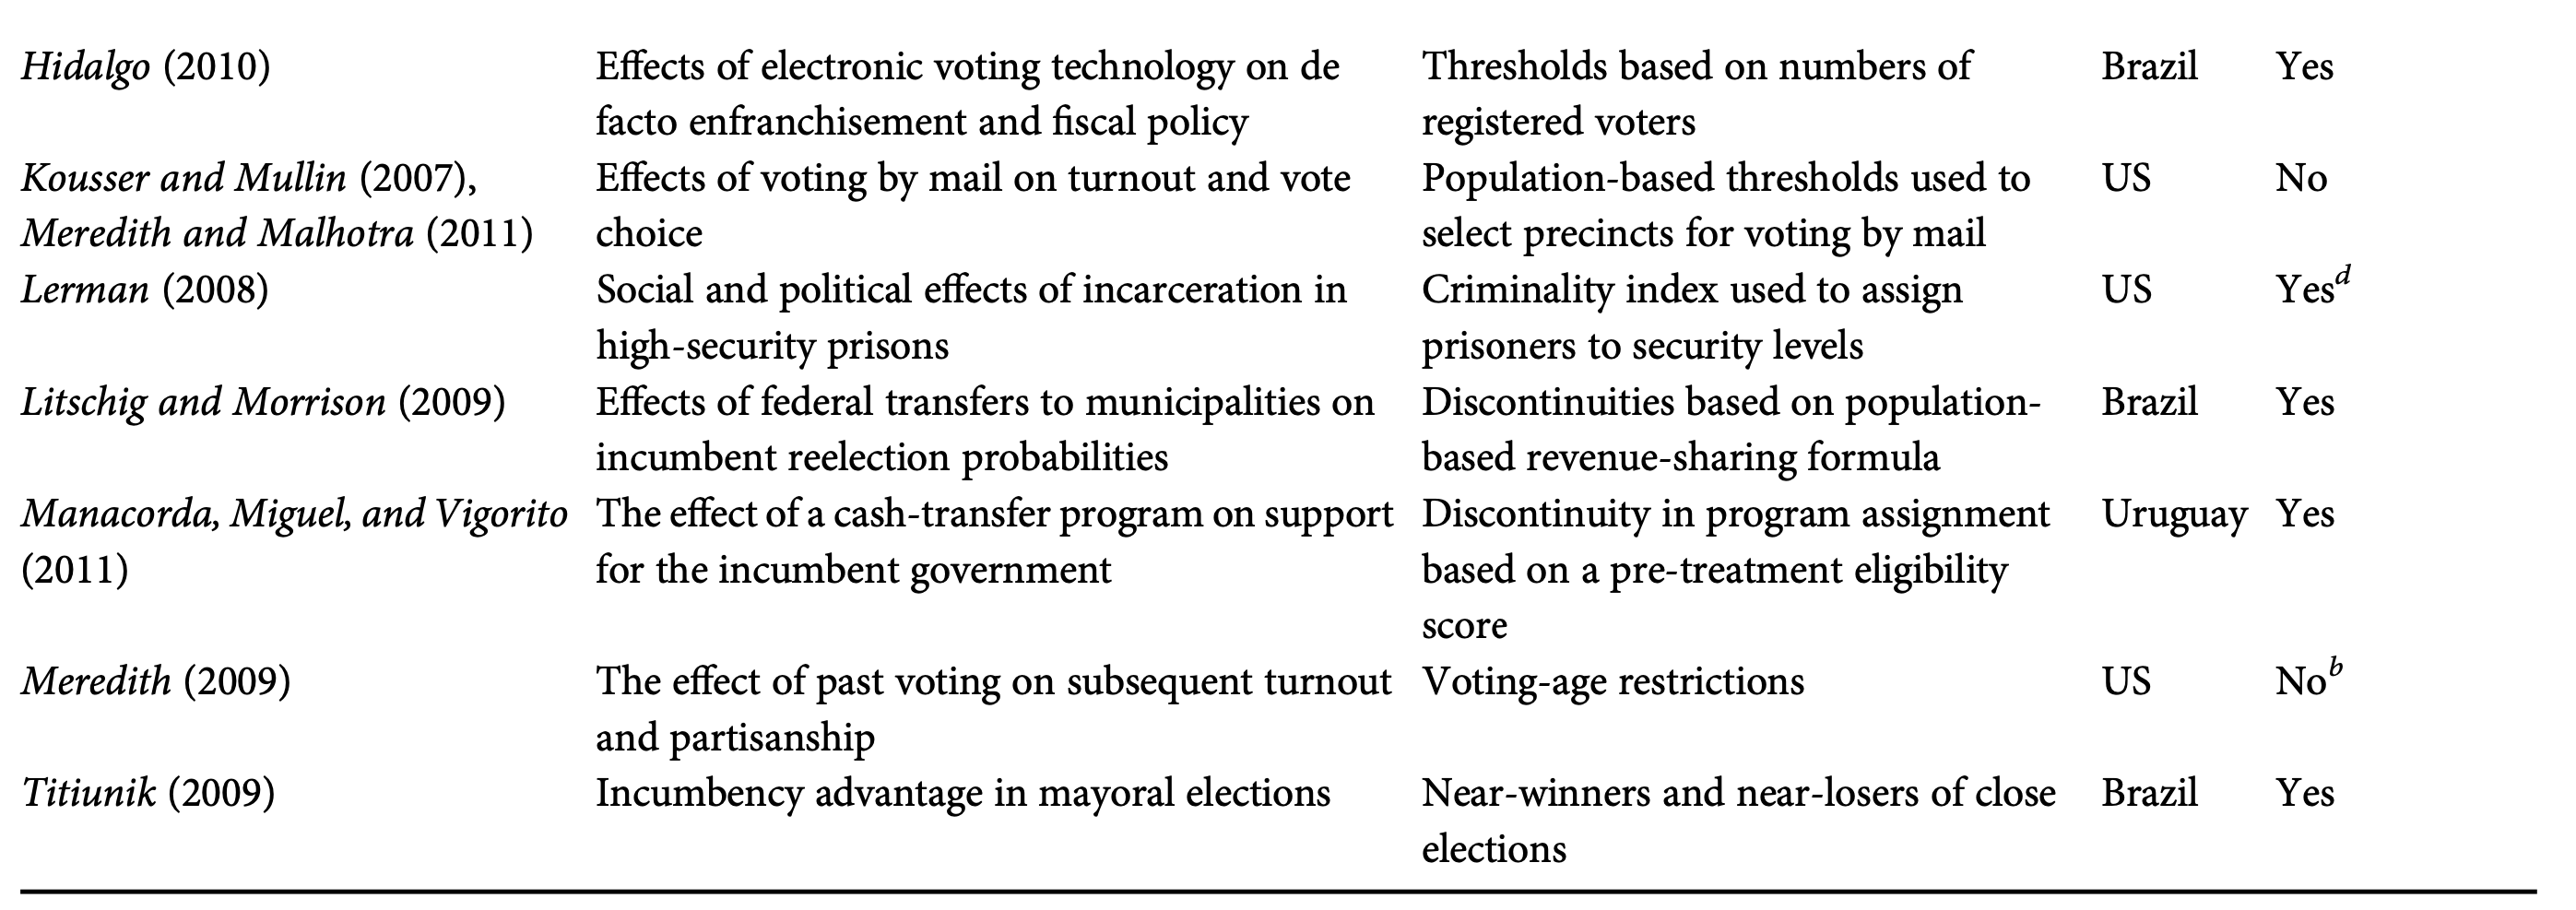
\includegraphics{figs/nat_exp_RDD3.png}
\end{frame}

\begin{frame}{Diseños de Variables Instrumentales: fuente de la VI}
\protect\hypertarget{diseuxf1os-de-variables-instrumentales-fuente-de-la-vi}{}
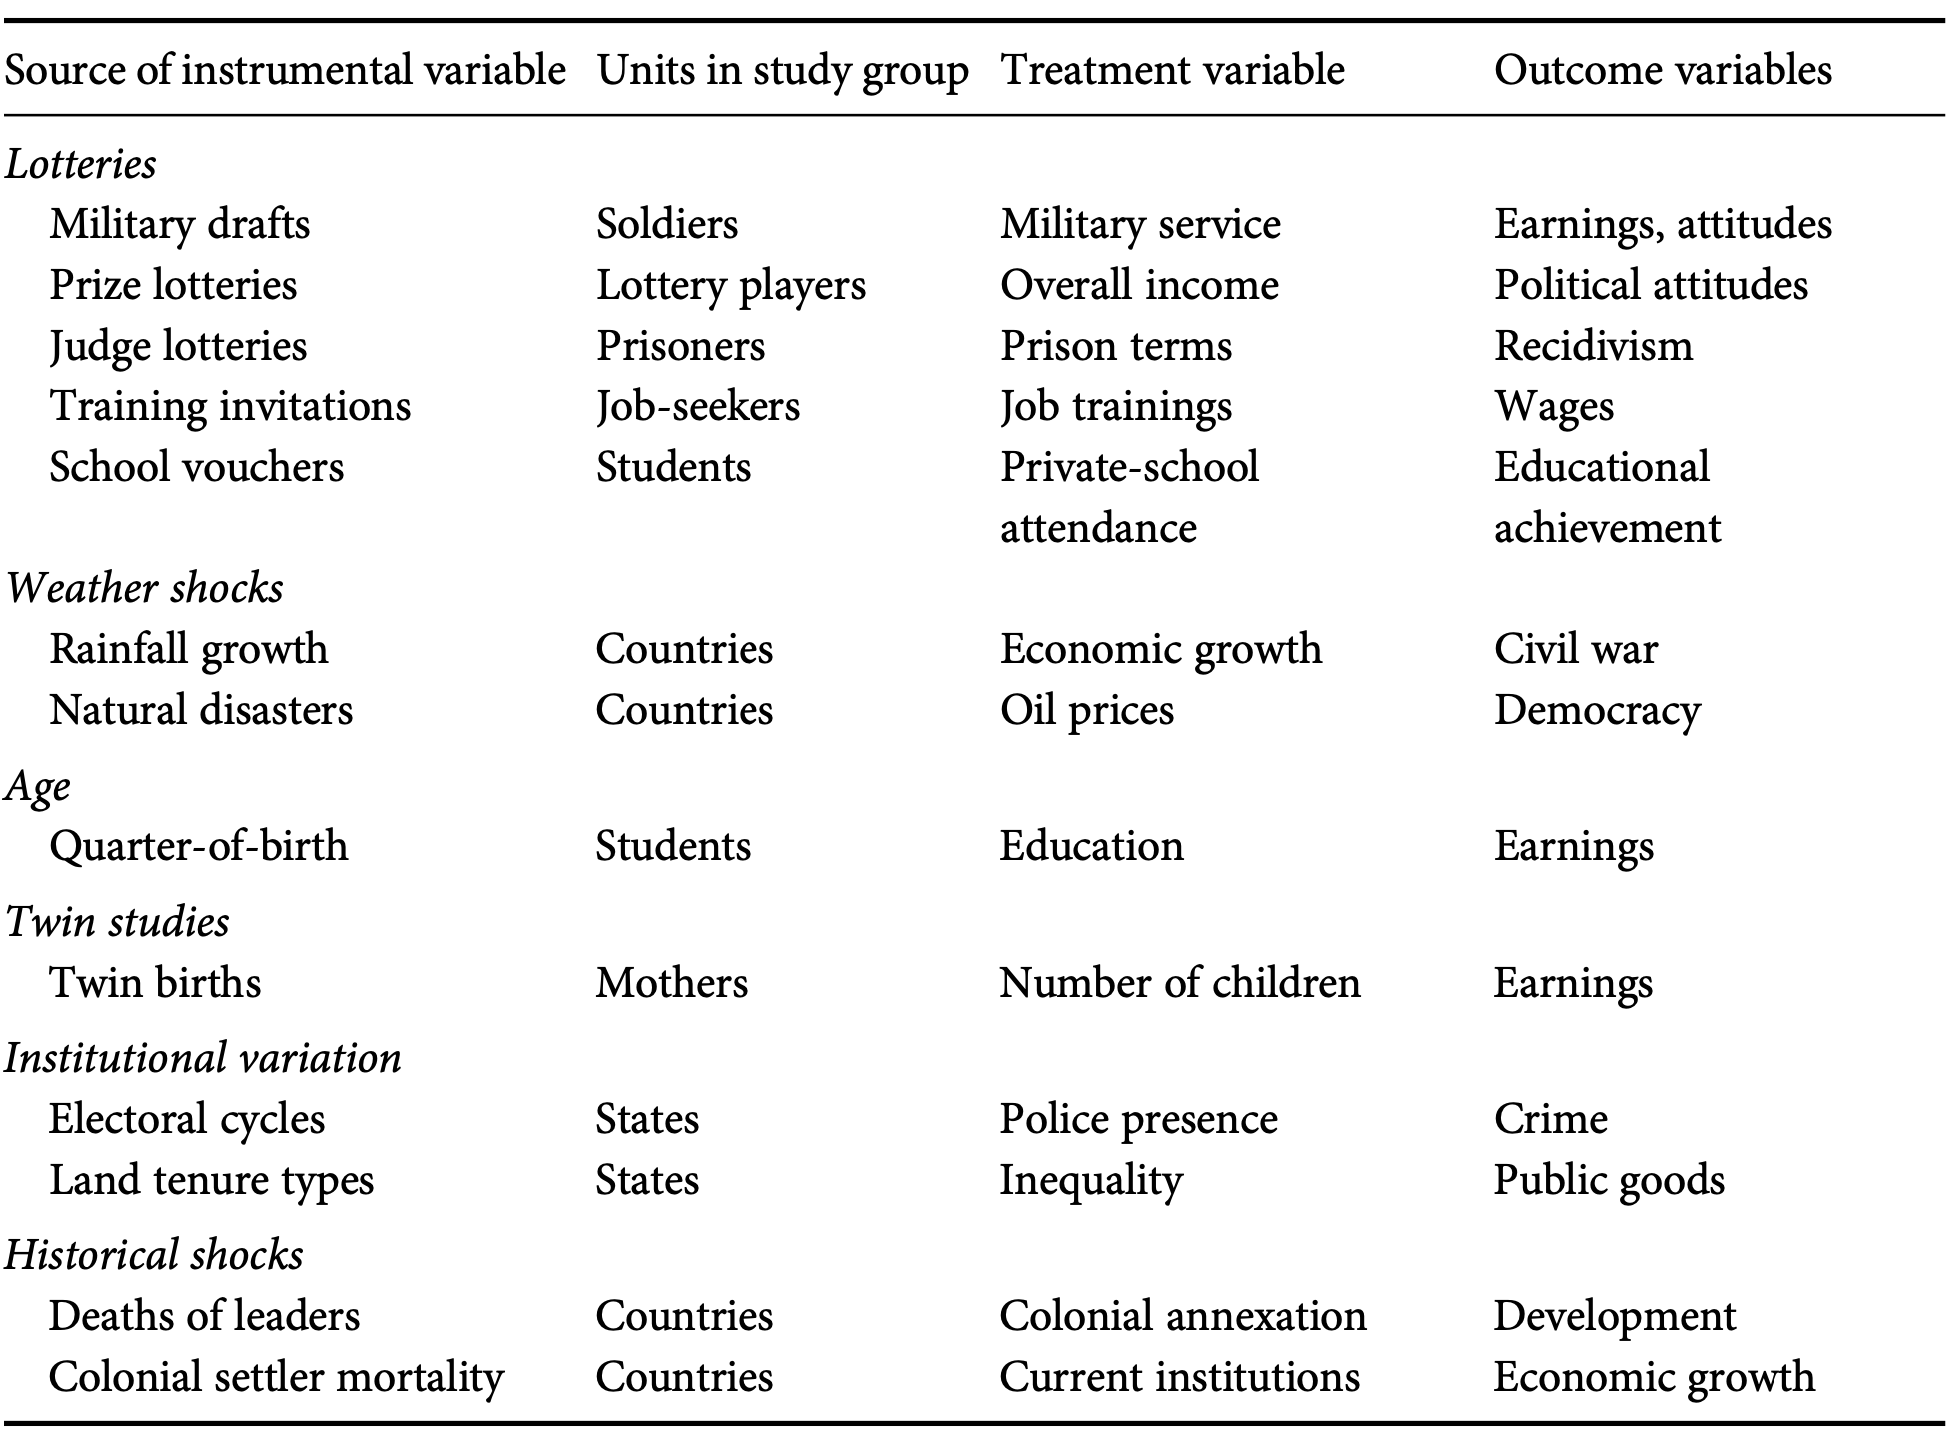
\includegraphics{figs/nat_exp_IV1.png}
\end{frame}

\begin{frame}{Diseños de Variables Instrumentales: Ejemplos}
\protect\hypertarget{diseuxf1os-de-variables-instrumentales-ejemplos}{}
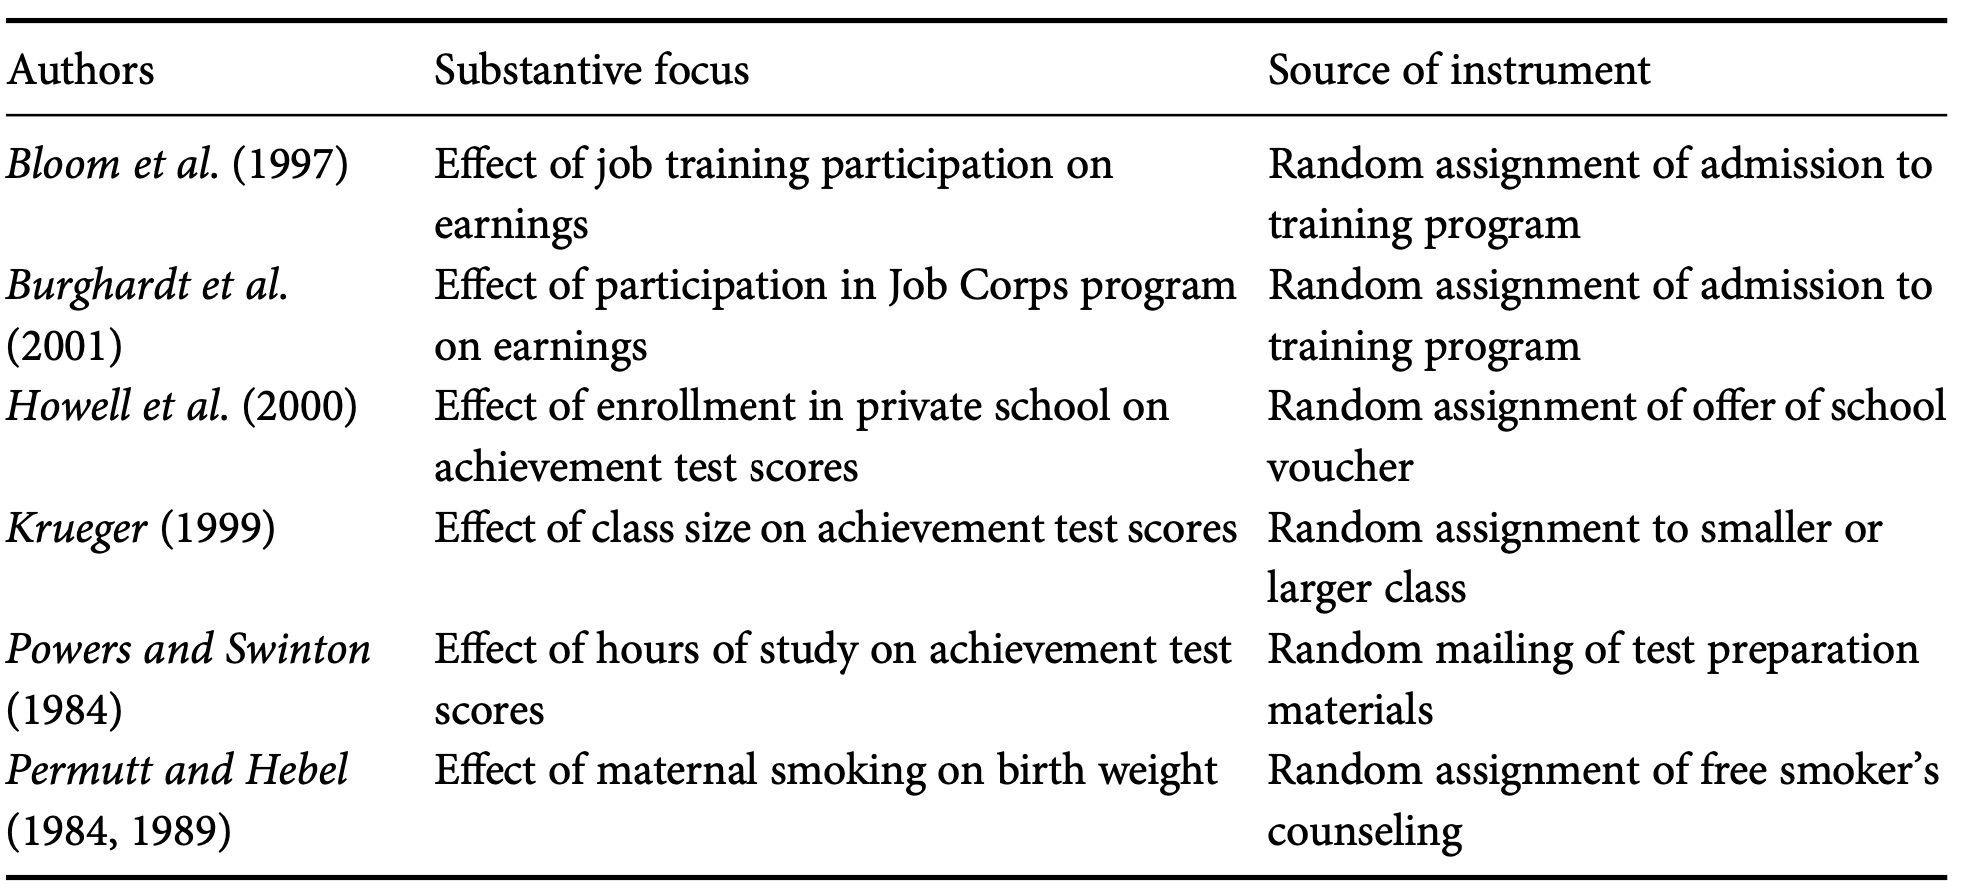
\includegraphics{figs/nat_exp_IV2.png}
\end{frame}

\begin{frame}{Evaluando Experimentos Naturales: limitaciones}
\protect\hypertarget{evaluando-experimentos-naturales-limitaciones}{}
\begin{itemize}
\item
  Su uso conlleva retos analíticos específicos
\item
  Evaluando el ``as-if random'':

  \begin{itemize}
  \tightlist
  \item
    Tests de balance
  \item
    Diagnósticos cualitativos
  \end{itemize}
\item
  Dado que no se planificados sino descubiertos, el uso de experimentos
  naturales para un determinado programa de investigación implica un
  elemento de suerte
\end{itemize}
\end{frame}

\begin{frame}{Plausibility of as-if random assignment}
\protect\hypertarget{plausibility-of-as-if-random-assignment}{}
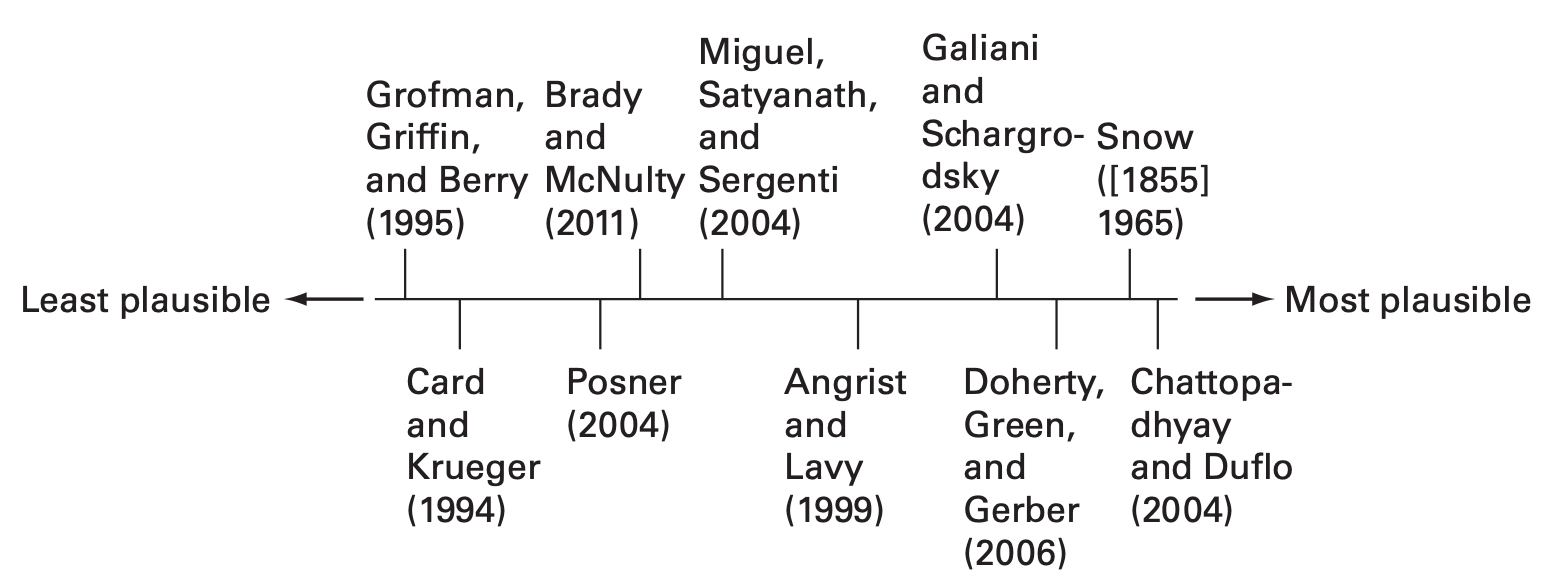
\includegraphics{figs/plausibility.png}
\end{frame}

\begin{frame}{Relevancia de la intervención}
\protect\hypertarget{relevancia-de-la-intervenciuxf3n}{}
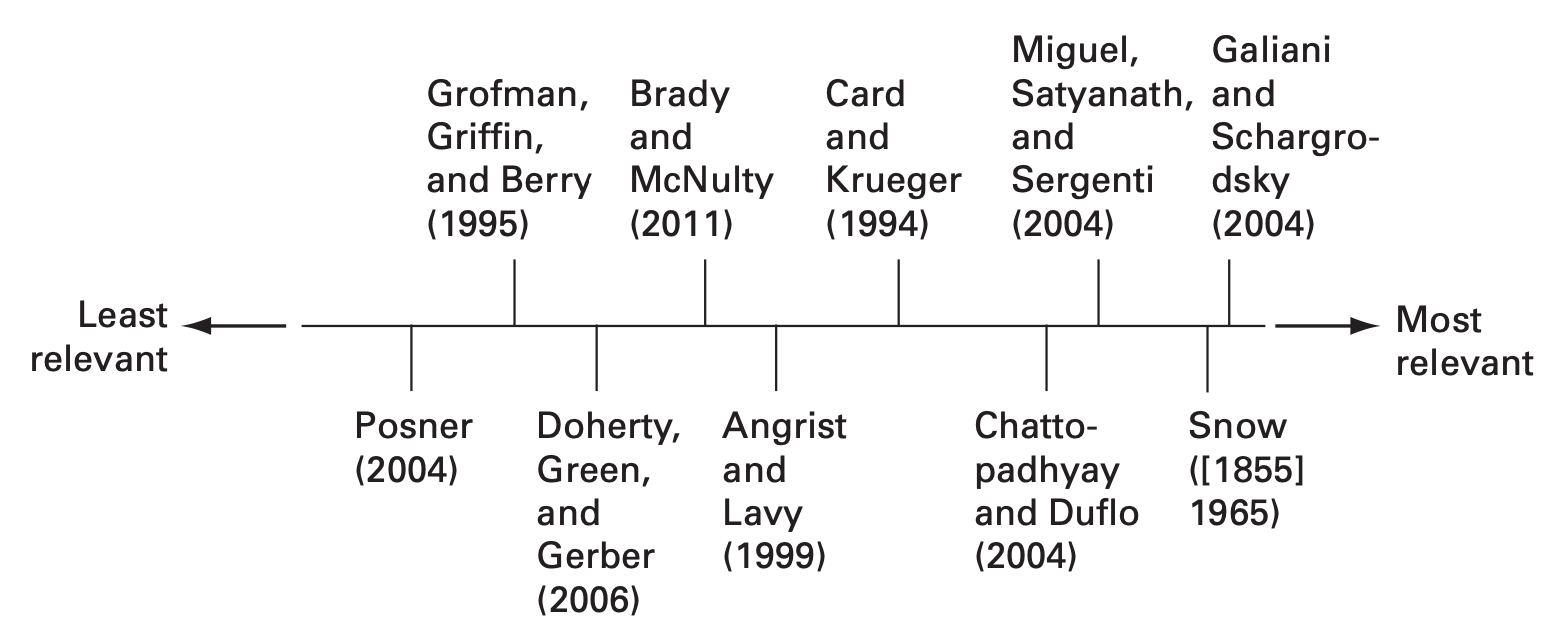
\includegraphics{figs/relevance.png}
\end{frame}

\begin{frame}{Fortaleza de los diseños}
\protect\hypertarget{fortaleza-de-los-diseuxf1os}{}
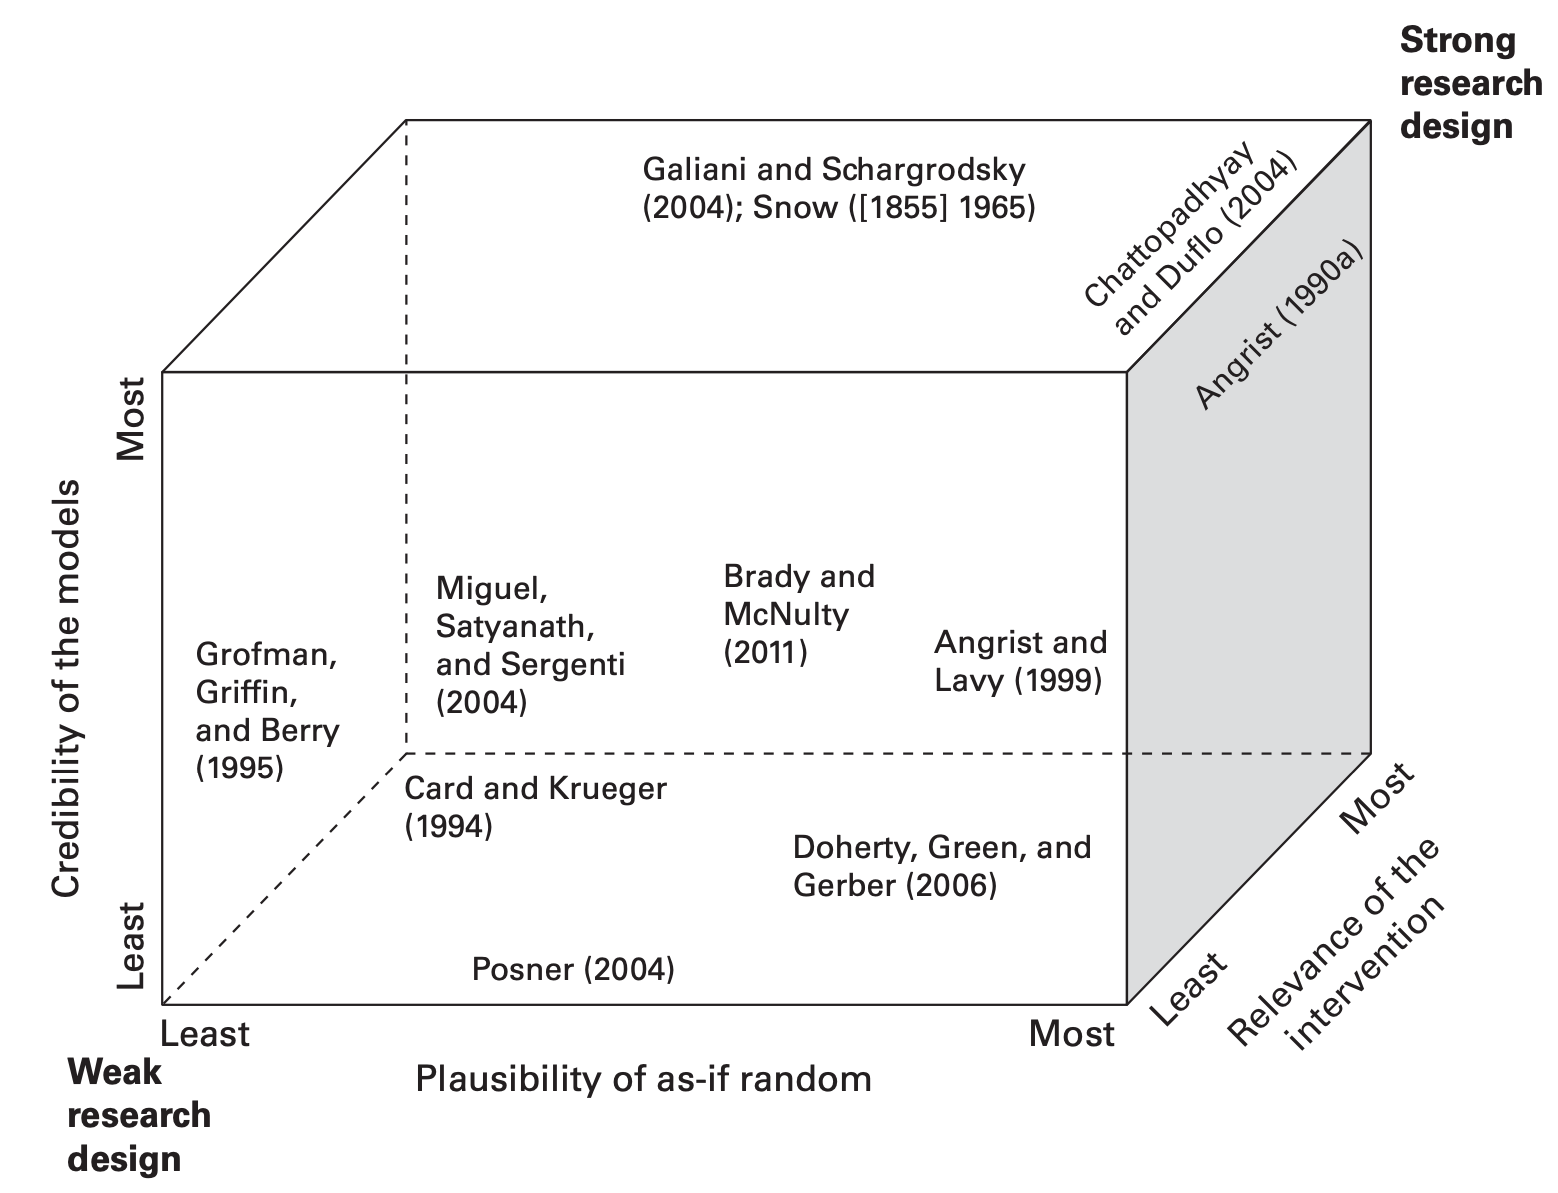
\includegraphics{figs/strength.png}
\end{frame}

\hypertarget{experimentos-de-encuesta}{%
\section{Experimentos de Encuesta}\label{experimentos-de-encuesta}}

\begin{frame}{Lecturas}
\protect\hypertarget{lecturas-2}{}
\begin{itemize}
\item
  Gaines, Brian J., James H. Kuklinski, and Paul J. Quirk. 2007. ``The
  Logic of the Survey Experiment Reexamined.'' Political Analysis
  15(01): 1--20.
\item
  Coppock, Alexander. 2018. ``Generalizing from Survey Experiments
  Conducted on Mechanical Turk: A Replication Approach.'' Political
  Science Research and Methods (2015): 1--16.
\item
  Tobergte, David R., and Shirley Curtis. 2013. ``The Generalizability
  of Survey Experiments.'' Journal of Chemical Information and Modeling
  53(9): 1689--99.
\end{itemize}
\end{frame}

\begin{frame}{Actividad}
\protect\hypertarget{actividad}{}
\begin{enumerate}
\tightlist
\item
  Tomen un papel
\item
  No digan el número que les tocó
\item
  Grupo 2, cierren los ojos
\end{enumerate}
\end{frame}

\begin{frame}{Actividad}
\protect\hypertarget{actividad-1}{}
Grupo 1

Piensen si la población de Chicago es mayor o menor a 500.000
habitantes.

¿Cuál crees que es la población de Chicago?
\end{frame}

\begin{frame}{Actividad}
\protect\hypertarget{actividad-2}{}
Grupo 1, cierren los ojos
\end{frame}

\begin{frame}{Actividad}
\protect\hypertarget{actividad-3}{}
Grupo 2

Piensen si la población de Chicago es mayor o menor a 10.000.000
habitantes.

¿Cuál crees que es la población de Chicago?
\end{frame}

\begin{frame}{Ingresar los datos}
\protect\hypertarget{ingresar-los-datos}{}
Vayan a: \url{https://bit.ly/2Sxsp17}

Ingresen creencia y su número de grupo
\end{frame}

\begin{frame}{Resultados}
\protect\hypertarget{resultados}{}
\begin{itemize}
\item
  Población verdadera: 2.79 millones
\item
  Ver resultados
\end{itemize}
\end{frame}

\begin{frame}{El primer experimento de encuesta}
\protect\hypertarget{el-primer-experimento-de-encuesta}{}
Hadley Cantril (1940) le preguntó a 3000 Americanos

Piensas que U.S. debería hacer más de lo que está haciendo actualmente
para ayudar a Inglaterra y Francia?

\begin{itemize}
\tightlist
\item
  Si
\item
  No
\end{itemize}
\end{frame}

\begin{frame}{El primer experimento de encuesta}
\protect\hypertarget{el-primer-experimento-de-encuesta-1}{}
Hadley Cantril (1940) le preguntó a 3000 Americanos

Piensas que U.S. debería hacer más de lo que está haciendo actualmente
para ayudar a Inglaterra y Francia?

\begin{itemize}
\tightlist
\item
  Si
\item
  No
\end{itemize}

Piensas que U.S. debería hacer más de lo que está haciendo actualmente
para ayudar a Inglaterra y Francia \textbf{en su pelea contra Hitler}?

\begin{itemize}
\tightlist
\item
  Si
\item
  No
\end{itemize}
\end{frame}

\begin{frame}{El primer experimento de encuesta}
\protect\hypertarget{el-primer-experimento-de-encuesta-2}{}
Hadley Cantril (1940) le preguntó a 3000 Americanos

Piensas que U.S. debería hacer más de lo que está haciendo actualmente
para ayudar a Inglaterra y Francia?

\begin{itemize}
\tightlist
\item
  Si 13\%
\item
  No
\end{itemize}

Piensas que U.S. debería hacer más de lo que está haciendo actualmente
para ayudar a Inglaterra y Francia \textbf{en su pelea contra Hitler}?

\begin{itemize}
\tightlist
\item
  Si 22\%
\item
  No
\end{itemize}

El ``efecto Hitler'' fue 22\% - 13\% = 9\%
\end{frame}

\begin{frame}{¿Qué son los Experimentos de Encuesta?}
\protect\hypertarget{quuxe9-son-los-experimentos-de-encuesta}{}
\begin{itemize}
\item
  Experimento realizado dentro de una encuesta
\item
  Dos tipos de experimentos de encuesta:

  \begin{itemize}
  \tightlist
  \item
    Para medir actitudes o comportamientos sensibles
  \item
    Para aprender sobre relaciones causales.
  \end{itemize}
\end{itemize}
\end{frame}

\begin{frame}{Experimentos de encuesta para medir temas sensibles}
\protect\hypertarget{experimentos-de-encuesta-para-medir-temas-sensibles}{}
\begin{itemize}
\tightlist
\item
  Temas sensibles: cualquier actitud o comportamiento con el que el
  encuestado no quiere que se le asocie públicamente
\item
  Intentan proporcionar anonimato a los encuestados para que puedan
  expresar actitudes potencialmente delicadas sin ser identificados
\end{itemize}
\end{frame}

\begin{frame}{Experimentos de Lista}
\protect\hypertarget{experimentos-de-lista}{}
\begin{itemize}
\tightlist
\item
  Se asigna aleatoriamente a los encuestados a una condición de control
  o de tratamiento:

  \begin{itemize}
  \tightlist
  \item
    Control: presenta a los encuestados una lista de elementos
  \item
    Tratamiento: presenta la misma lista más un elemento de tratamiento
    que mide la actitud o el comportamiento de interés.
  \end{itemize}
\item
  Se pregunta a los encuestados cuántos de esos ítems se aplican a su
  caso.
\end{itemize}
\end{frame}

\begin{frame}{Ejemplo: Experimentos de Lista}
\protect\hypertarget{ejemplo-experimentos-de-lista}{}
Kuklinski et al.~(1997) estudiaron la discriminación racial con un
experimento de listas de encuestas.

Ahora voy a leerle cosas que a veces enfadan o molestan a la gente.
Después de que las lea, dígame \textbf{CUÁNTAS} de ellas le molestan. No
quiero saber cuáles, sólo \textbf{CUÁNTAS}.

\begin{enumerate}
\tightlist
\item
  Que el gobierno federal aumente el impuesto sobre la gasolina
\item
  Los contratos millonarios de los deportistas profesionales
\item
  Grandes empresas que contaminan el medio ambiente
\end{enumerate}
\end{frame}

\begin{frame}{Ejemplo: Experimentos de Lista}
\protect\hypertarget{ejemplo-experimentos-de-lista-1}{}
Kuklinski et al.~(1997) estudiaron la discriminación racial con un
experimento de listas de encuestas.

Ahora voy a leerle cosas que a veces enfadan o molestan a la gente.
Después de que las lea, dígame \textbf{CUÁNTAS} de ellas le molestan. No
quiero saber cuáles, sólo \textbf{CUÁNTAS}.

\begin{enumerate}
\tightlist
\item
  Que el gobierno federal aumente el impuesto sobre la gasolina
\item
  Los contratos millonarios de los deportistas profesionales
\item
  Grandes empresas que contaminan el medio ambiente
\item
  \textbf{Una familia negra que se muda a la casa de al lado}
\end{enumerate}
\end{frame}

\begin{frame}{Ejemplo: Experimentos de Lista}
\protect\hypertarget{ejemplo-experimentos-de-lista-2}{}
\begin{itemize}
\tightlist
\item
  La media de ítems elegidos en el grupo de tratamiento fue de 2,37
\item
  La media de ítems elegidos en el grupo de control fue de 1,95
\item
  La diferencia de 0,42 entre el grupo de tratamiento y el de control
  indica que al 42 porciento de los encuestados les molestaría que una
  familia negra se mudara a la casa de al lado.
\end{itemize}
\end{frame}

\begin{frame}{Experimentos de Respuesta aleatoria}
\protect\hypertarget{experimentos-de-respuesta-aleatoria}{}
\begin{itemize}
\tightlist
\item
  También se utiliza para medir una actitud o comportamiento sensible
\item
  Utiliza un dispositivo de aleatorización para dictar si el encuestado
  debe responder a la pregunta delicada o a otra cosa
\end{itemize}
\end{frame}

\begin{frame}{Ejemplo Experimentos de Respuesta
aleatoria\footnote<.->{Blair, Imai y Zhou (2015) ``Design and Analysis
  of the Randomized Response Technique.'' JASA 110(511): 1304--19.}}
\protect\hypertarget{ejemplo-experimentos-de-respuesta-aleatoria}{}
Aquí hay una bolsa; en ella hay piedras del juego `Go', algunas de color
negro y otras blancas. Por favor, saca una piedra y mira de qué color
es, blanca o negra. No me digas si es negra o blanca, pero asegúrate de
saber cuál es.

Si coge una \textbf{negra}, responda a la pregunta: ``¿Ha tenido alguna
vez un aborto inducido?''

Si coge una \textbf{blanca}, responda a la pregunta: ``¿Nació usted en
el año lunar del caballo?''

Consideraciones:

\begin{itemize}
\tightlist
\item
  Puede utilizar cualquier dispositivo de aleatorización
\item
  Puede ser cognitivamente complejo
\end{itemize}
\end{frame}

\begin{frame}{Experimentos de encuesta para medir relaciones causales}
\protect\hypertarget{experimentos-de-encuesta-para-medir-relaciones-causales}{}
Los experimentos de encuestas para medir relaciones causales son como
cualquier otro experimento, salvo que la intervención experimental y la
medición de resultados se producen en el contexto de una encuesta.
\end{frame}

\begin{frame}{Diseños de viñeta}
\protect\hypertarget{diseuxf1os-de-viuxf1eta}{}
\begin{itemize}
\tightlist
\item
  Una viñeta es un texto corto que describe una situación
\item
  Se proporciona un escenario para que el encuestado lo lea, variando
  los componentes clave del escenario.
\end{itemize}
\end{frame}

\begin{frame}{Un ejemplo de viñeta\footnote<.->{Gilens, M. 1996. ```Race
  coding' andwhite opposition to welfare. American Political Science
  Review 90(3): 593--604.}}
\protect\hypertarget{un-ejemplo-de-viuxf1eta}{}
Ahora piensa en una mujer \textbf{(negra/blanca)} de treinta y pocos
años. \textbf{(Finalizó/Abandonó)} sus estudios de bachillerato, tiene
un hijo de diez años y lleva un año recibiendo ayudas sociales.

\begin{itemize}
\tightlist
\item
  ¿Qué probabilidad crees que hay de que tenga más hijos para recibir
  más ayudas sociales? (1 = Muy probable, \ldots, 7 = Nada probable)
\item
  ¿Qué probabilidad crees que hay de que se esfuerce de verdad por
  encontrar trabajo el año que viene? (1 = Muy probable, \ldots, 7 =
  Nada probable)
\end{itemize}
\end{frame}

\begin{frame}{Tratamientos no textuales\footnote<.->{Iyengar et
  al.~2010. ``Do Explicit Racial Cues Influence Candidate Preference?
  The Case of Skin Complexion in the 2008 Campaign.'\,' Working paper.}}
\protect\hypertarget{tratamientos-no-textuales}{}
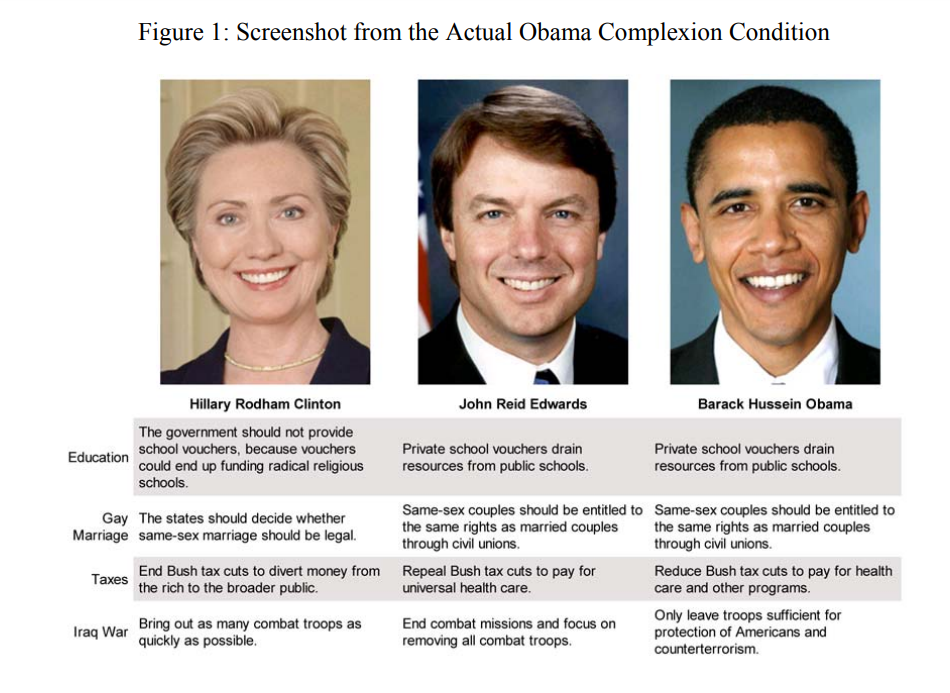
\includegraphics{figs/Iyengar et al. 2010_figure 1.PNG}
\end{frame}

\begin{frame}{Tratamientos no textuales\footnote<.->{Iyengar et
  al.~2010. ``Do Explicit Racial Cues Influence Candidate Preference?
  The Case of Skin Complexion in the 2008 Campaign.'\,' Working paper.}}
\protect\hypertarget{tratamientos-no-textuales-1}{}
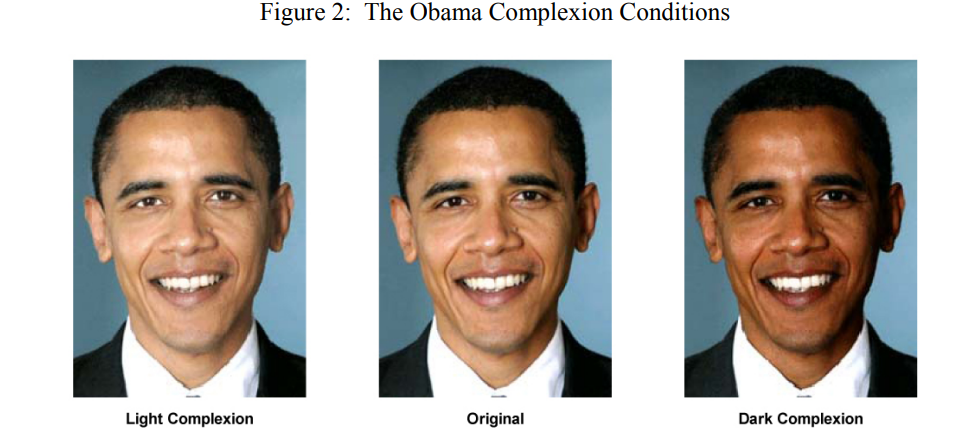
\includegraphics{figs/Iyengar et al. 2010_figure 2.PNG}
\end{frame}

\begin{frame}{Manipulación de Audio y Videos}
\protect\hypertarget{manipulaciuxf3n-de-audio-y-videos}{}
\begin{itemize}
\tightlist
\item
  Problemático por la misma razón que los textos largos
\item
  Mejores prácticas

  \begin{itemize}
  \tightlist
  \item
    Que sea breve
  \item
    Hacer que el vídeo se reproduzca automáticamente
  \item
    Deshabilitar la progresión de la encuesta
  \item
    Controlar y validar
  \end{itemize}
\item
  Ejemplos

  \begin{itemize}
  \tightlist
  \item
    Publicidad de televisión\footnote<.->{Vavreck. 2007 ``The
      Exaggerated Effects of Advertising on Turnout: The Dangers of
      Self-Reports.'\,' Quarterly Journal of Political Science 2:
      325--343.}
  \item
    Programas de noticias\footnote<.->{Mutz. 2007. ``Effects of
      `In-Your-Face' Television Discourse on Perceptions of a Legitimate
      Opposition.'' American Political Science Review 101(4): 621--635.}
  \end{itemize}
\end{itemize}
\end{frame}

\begin{frame}{Diseños de tareas}
\protect\hypertarget{diseuxf1os-de-tareas}{}
\begin{itemize}
\tightlist
\item
  Los diseños de tareas piden a los encuestados que realicen una tarea
\item
  Ejemplo más común: escribir algo
\item
  Puede ser problemático:

  \begin{itemize}
  \tightlist
  \item
    Intensivo en tiempo
  \item
    Invita a abandonar
  \item
    Problemas de cumplimiento
  \end{itemize}
\end{itemize}
\end{frame}

\begin{frame}{Diseños de tareas Ejemplo}
\protect\hypertarget{diseuxf1os-de-tareas-ejemplo}{}
Hoy en día, Demócratas y Republicanos difieren considerablemente entre
sí. Los dos grupos parecen cada vez más alejados, no sólo en sus
opiniones, sino también en sus estilos de vida. Al principio de la
encuesta, usted dijo que tiende a identificarse como
(demócrata/republicano). Tómese unos minutos para pensar qué le gusta de
los (demócratas/republicanos) en comparación con los
(republicanos/demócratas). Piense en 2 ó 3 cosas que le gusten
especialmente de \textbf{su partido}. A continuación, piensa en 2 ó 3
cosas que le disgustan especialmente del \textbf{otro partido}. Ahora,
por favor, escriba esos pensamientos en el espacio de abajo.
\end{frame}

\begin{frame}{Diseños de tareas Ejemplo}
\protect\hypertarget{diseuxf1os-de-tareas-ejemplo-1}{}
Hoy en día, Demócratas y Republicanos difieren considerablemente entre
sí. Los dos grupos parecen cada vez más alejados, no sólo en sus
opiniones, sino también en sus estilos de vida. Al principio de la
encuesta, usted dijo que tiende a identificarse como
(demócrata/republicano). Tómese unos minutos para pensar qué le gusta de
los (demócratas/republicanos) en comparación con los
(republicanos/demócratas). Piense en 2 ó 3 cosas que le gusten
especialmente de \textbf{el otro partido}. A continuación, piensa en 2 ó
3 cosas que le disgustan especialmente de \textbf{su partido}. Ahora,
por favor, escriba esos pensamientos en el espacio de abajo.
\end{frame}

\begin{frame}{Experimentos perfiles emparejados o conjoint}
\protect\hypertarget{experimentos-perfiles-emparejados-o-conjoint}{}
\begin{itemize}
\tightlist
\item
  Los experimentos conjoint consisten en medir las preferencias
  reveladas a partir de una serie de decisiones de elección forzada.
\item
  Los encuestados deben elegir entre dos ``perfiles'' distintos que
  contienen muchas características
\item
  Estimar la importancia relativa de las características de cada
  atributo (con respecto a una categoría de base)
\item
  Aleatorizar las características de los perfiles le otorga un
  significado causal a las preferncias entre los atributos
\end{itemize}
\end{frame}

\begin{frame}{Experimentos conjoint}
\protect\hypertarget{experimentos-conjoint}{}
Ventajas

\begin{itemize}
\tightlist
\item
  Imita decisiones del mundo real
\item
  Mayor potencia estadística
\item
  Interpertación causal de las preferencias reveladas
\end{itemize}

Desventajas

\begin{itemize}
\tightlist
\item
  Mayor complejidad cognitiva para los encuestados que las encuestas
  tradicionales
\item
  Los resultados de los experimentos conjuntos son difíciles de
  interpretar
\item
  Crean combinaciones poco realistas
\end{itemize}
\end{frame}

\begin{frame}{Ejemplo: Estudio sobre el apoyo a la
inmigración\footnote<.->{Hainmueller, Jens, and Daniel J. Hopkins. 2015.
  ``The Hidden American Immigration Consensus: A Conjoint Analysis of
  Attitudes toward Immigrants.'' American Journal of Political Science
  59 (3): 529--48}}
\protect\hypertarget{ejemplo-estudio-sobre-el-apoyo-a-la-inmigraciuxf3n}{}
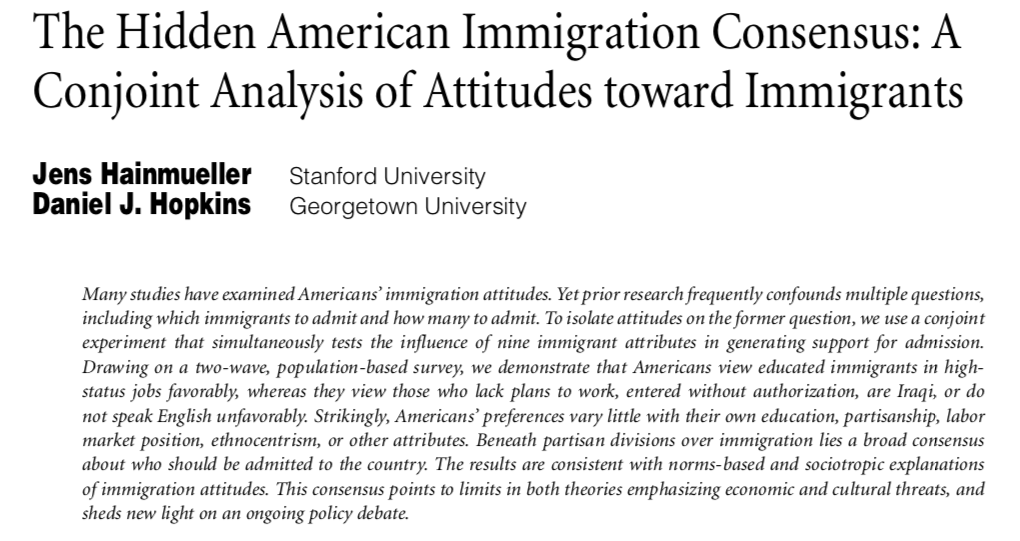
\includegraphics[width=0.8\textwidth,height=\textheight]{figs/Conjoint_1.PNG}
\end{frame}

\begin{frame}{Ejemplo: Estudio sobre el apoyo a la
inmigración\footnote<.->{Hainmueller, Jens, and Daniel J. Hopkins. 2015.
  ``The Hidden American Immigration Consensus: A Conjoint Analysis of
  Attitudes toward Immigrants.'' American Journal of Political Science
  59 (3): 529--48}}
\protect\hypertarget{ejemplo-estudio-sobre-el-apoyo-a-la-inmigraciuxf3n-1}{}
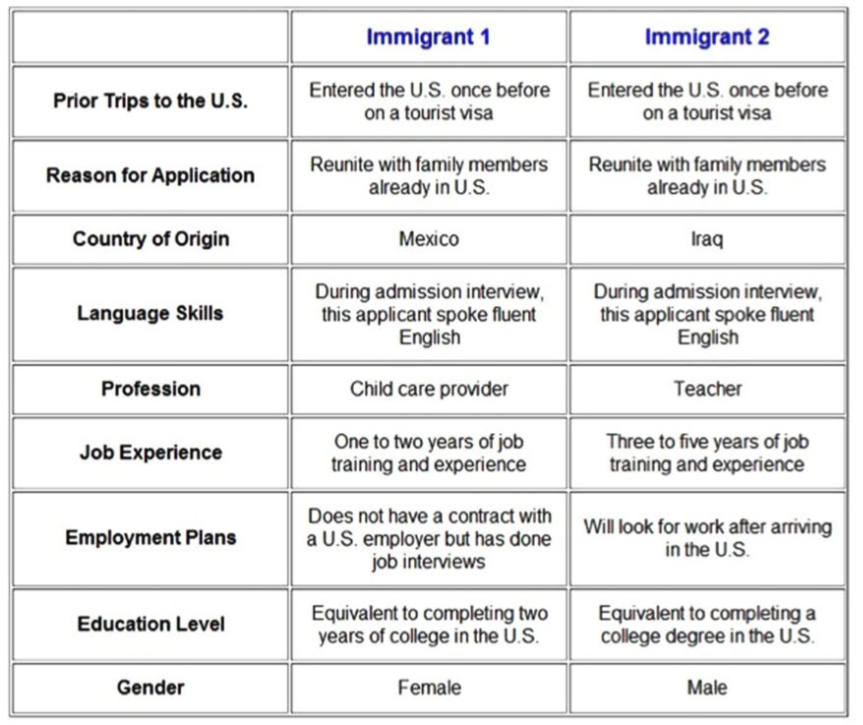
\includegraphics[width=0.8\textwidth,height=\textheight]{figs/inmigrant_profiles.png}
\end{frame}

\begin{frame}{Ejemplo: Estudio sobre el apoyo a la
inmigración\footnote<.->{Hainmueller, Jens, and Daniel J. Hopkins. 2015.
  ``The Hidden American Immigration Consensus: A Conjoint Analysis of
  Attitudes toward Immigrants.'' American Journal of Political Science
  59 (3): 529--48}}
\protect\hypertarget{ejemplo-estudio-sobre-el-apoyo-a-la-inmigraciuxf3n-2}{}
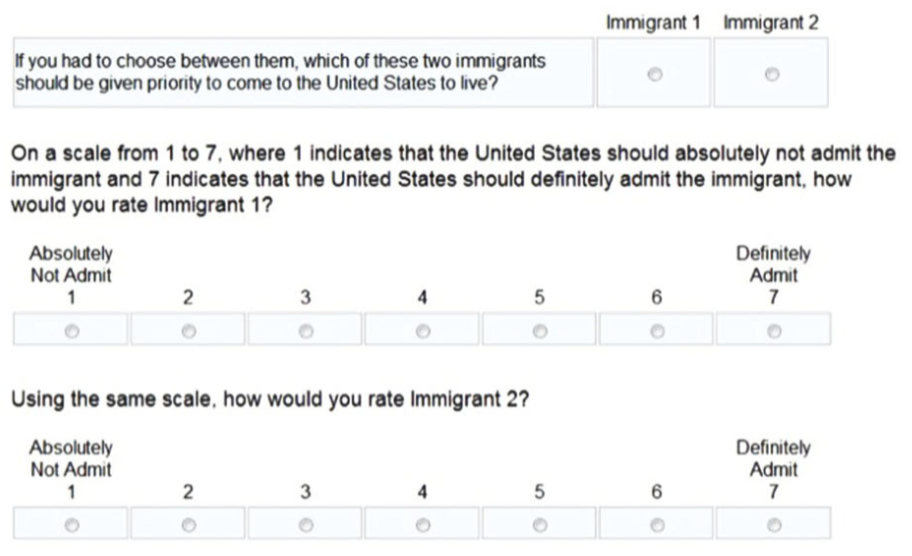
\includegraphics{figs/inmigrant_outcomes.png}
\end{frame}

\begin{frame}{Ejemplo: Estudio sobre el apoyo a la
inmigración\footnote<.->{Hainmueller, Jens, and Daniel J. Hopkins. 2015.
  ``The Hidden American Immigration Consensus: A Conjoint Analysis of
  Attitudes toward Immigrants.'' American Journal of Political Science
  59 (3): 529--48}}
\protect\hypertarget{ejemplo-estudio-sobre-el-apoyo-a-la-inmigraciuxf3n-3}{}
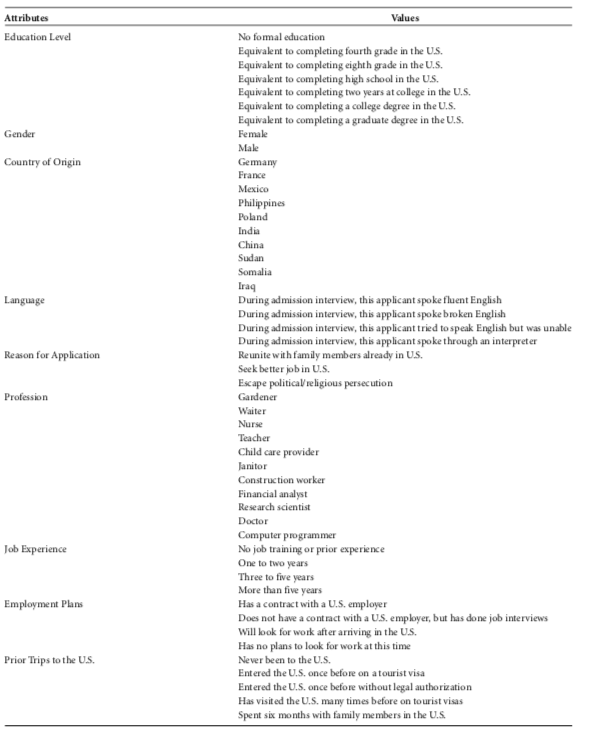
\includegraphics[width=0.7\textwidth,height=\textheight]{figs/conjoint_table.PNG}
\end{frame}

\begin{frame}{Ejemplo: Estudio sobre el apoyo a la inmigración -
Resultados\footnote<.->{Hainmueller, Jens, and Daniel J. Hopkins. 2015.
  ``The Hidden American Immigration Consensus: A Conjoint Analysis of
  Attitudes toward Immigrants.'' American Journal of Political Science
  59 (3): 529--48}}
\protect\hypertarget{ejemplo-estudio-sobre-el-apoyo-a-la-inmigraciuxf3n---resultados}{}
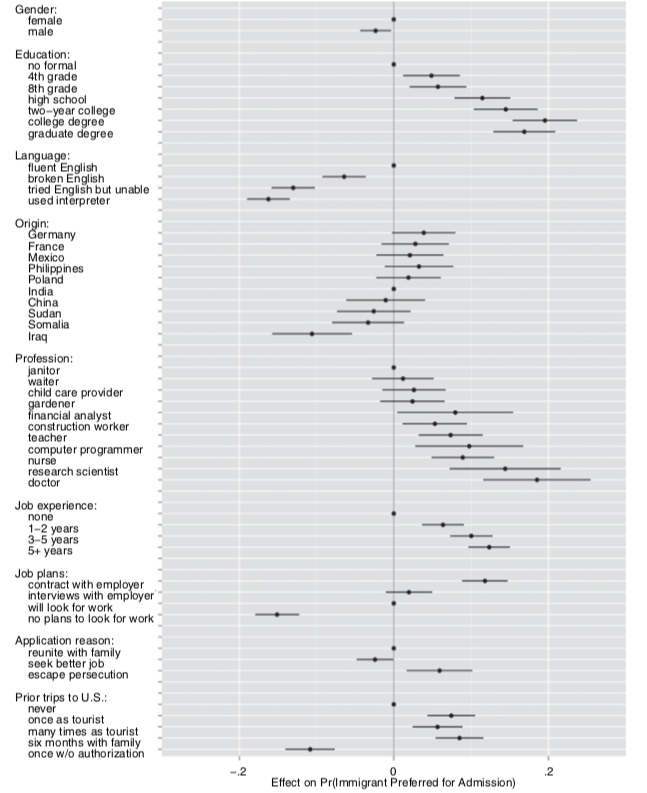
\includegraphics[width=0.6\textwidth,height=\textheight]{figs/conjoint_results.PNG}
\end{frame}

\begin{frame}{AMCE (Average Marginal Component Effect)\footnote<.->{Hainmueller,
  J., Hopkins, D., \& Yamamoto, T. (2014). ``Causal Inference in
  Conjoint Analysis: Understanding Multidimensional Choices via Stated
  Preference Experiments.'' Political Analysis, 22(1)}}
\protect\hypertarget{amce-average-marginal-component-effect}{}
Efecto marginal del atributo l sobre el promedio de la distribución
conjunta de los atributos restantes

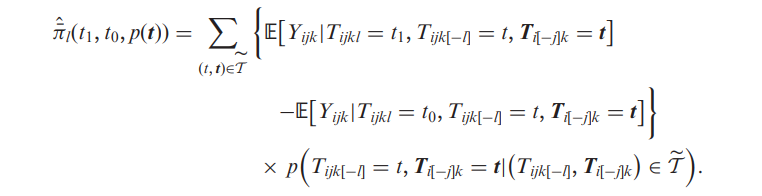
\includegraphics{figs/AMCE_2.PNG}
\end{frame}

\begin{frame}{Manipulation Check}
\protect\hypertarget{manipulation-check}{}
¿Cómo sabemos que estamos manipulando lo que creemos que estamos
manipulando?

\begin{itemize}
\tightlist
\item
  Una opción: usando manipulation checks

  \begin{itemize}
  \tightlist
  \item
    Se utilizan para comprobar si la manipulación realizada en un
    experimento es percibida por los sujetos como el investigador desea
    que sea percibida
  \end{itemize}
\end{itemize}
\end{frame}

\begin{frame}{Manipulation Check\footnote<.->{Kane, J and Barabas, J.
  2019. ``A Note on Dropping Experimental Subjects Who Fail a
  Manipulation Check.'' American Journal of Political Science 36(1):
  234--249.}}
\protect\hypertarget{manipulation-check-1}{}
\begin{itemize}
\tightlist
\item
  Subjective manipulation check

  \begin{itemize}
  \tightlist
  \item
    Preguntar a los encuestados su opinión sobre la variable
    independiente manipulada por el investigador
  \item
    No es posible que los individuos den una respuesta errónea
  \end{itemize}
\item
  Instructional Manipulation Checks

  \begin{itemize}
  \tightlist
  \item
    Técnica que intenta evaluar directamente la atención
  \item
    No guarda relación con el experimento\\
  \item
    No miden la atención en el tratamiento
  \end{itemize}
\item
  Factual Manipulation Checks

  \begin{itemize}
  \tightlist
  \item
    Una única pregunta que se formula a todos los participantes en el
    experimento
  \item
    Los FMC son MC que aparecen después del tratamiento y son
    pertinentes para la parte experimental de la encuesta (como los
    SMC), pero que también tienen opciones de respuesta correcta (como
    los IMC).
  \end{itemize}
\end{itemize}
\end{frame}

\begin{frame}{Manipulation Check\footnote<.->{Kane, J and Barabas, J.
  2019. ``A Note on Dropping Experimental Subjects Who Fail a
  Manipulation Check.'' American Journal of Political Science 36(1):
  234--249.}}
\protect\hypertarget{manipulation-check-2}{}
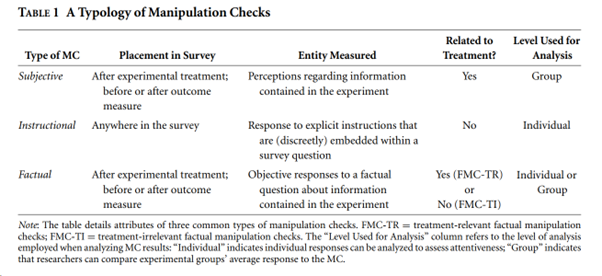
\includegraphics{figs/manipulation_checks_typology.png}
\end{frame}

\begin{frame}{Subjective Manipulation Check}
\protect\hypertarget{subjective-manipulation-check}{}
Al investigar si un servicio militar obligatorio nacional afectaría al
apoyo de los estadounidenses a ir a la guerra, Horowitz y Levendusky
(2011) intentan manipular las percepciones sobre el restablecimiento del
servicio militar obligatorio.

\begin{itemize}
\tightlist
\item
  El MC de los autores pide a los encuestados que ``evalúen la
  probabilidad de que se reintroduzca el servicio militar obligatorio
  utilizando una escala de respuesta de orden de 5 puntos que va de `muy
  improbable' a `muy probable'\,''.

  \begin{itemize}
  \tightlist
  \item
    Las respuestas a este ítem son intrínsecamente subjetiva
  \item
    Si el tratamiento es eficaz, los grupos de tratamiento deberían, en
    promedio, considerar más probable el restablecimiento del servicios
    militar obligatorio que el grupo de control.
  \end{itemize}
\end{itemize}
\end{frame}

\begin{frame}{Instructional Manipulation Check\footnote<.->{Oppenheimer,
  D.M. et al.~2009. ``Instructional manipulation checks: Detecting
  satisficing to increase statistical power.'' Journal of Experimental
  Social Psychology 45: 867--872.}}
\protect\hypertarget{instructional-manipulation-check}{}
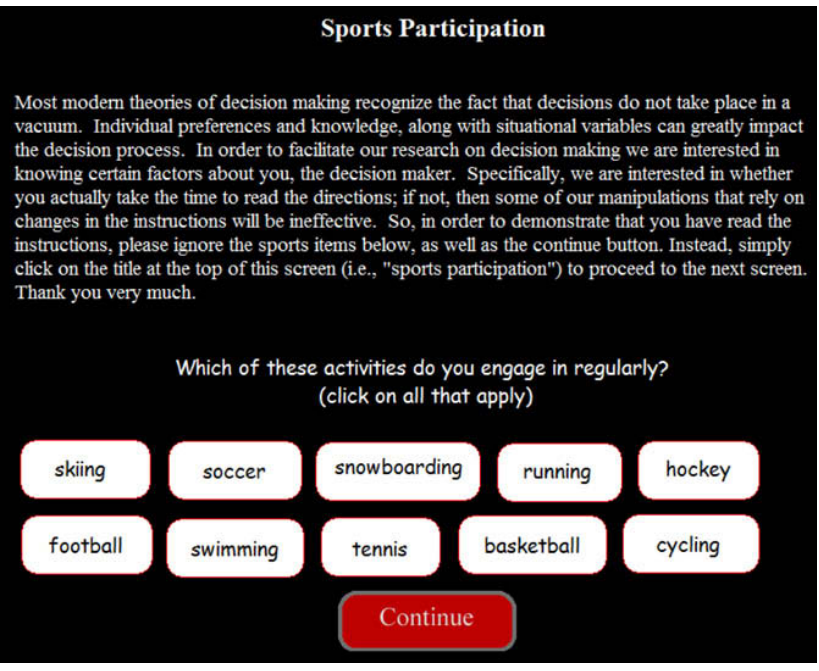
\includegraphics[width=0.8\textwidth,height=\textheight]{figs/IMC.PNG}
\end{frame}

\begin{frame}{Instructional Manipulation Check}
\protect\hypertarget{instructional-manipulation-check-1}{}
¿Está de acuerdo o en desacuerdo con la decisión de enviar fuerzas
británicas a luchar contra el ISIL en Siria? Nos gustaría saber si estás
leyendo las preguntas de esta encuesta. Si está leyendo atentamente,
ignore esta pregunta, no seleccione ninguna respuesta y haga clic en
``siguiente'' para continuar con la encuesta.

\begin{itemize}
\tightlist
\item
  Totalmente en desacuerdo
\item
  Algo en desacuerdo
\item
  Ni de acuerdo ni en desacuerdo
\item
  Algo de acuerdo
\item
  Totalmente de acuerdo
\end{itemize}
\end{frame}

\begin{frame}{Factual Manipulation Check\footnote<.->{Turner, J. 2007.
  ``The Messenger Overwhelming the Message: Ideological Cues and
  Perceptions of Bias in Television News.''Political Behavior 29(4):
  441--64.}}
\protect\hypertarget{factual-manipulation-check}{}
Turner (2007) manipula si varias noticias se atribuyen a la CNN o al Fox
News Channel, y así pide a todos los encuestados del estudio que
indiquen ``qué cadena produjo las noticias que vieron''.
\end{frame}

\begin{frame}{Manipulation Check: Mejores prácticas}
\protect\hypertarget{manipulation-check-mejores-pruxe1cticas}{}
\begin{itemize}
\tightlist
\item
  Los controles de manipulación deben ser inocuos:

  \begin{itemize}
  \tightlist
  \item
    No deben modificar la variable independiente
  \item
    No deben modificar la variable de resultado
  \end{itemize}
\item
  En general, medirlo después del outcome
\item
  Medir tanto lo que se quería manipular como lo que no se quería
  manipular
\end{itemize}
\end{frame}

\begin{frame}{Information Equivalence\footnote<.->{Dafoe, A., Zhang, B.,
  \& Caughey, D. (2018). ``Information Equivalence in Survey
  Experiments.'' Political Analysis, 26(4), 399-416.}}
\protect\hypertarget{information-equivalence}{}
\begin{itemize}
\tightlist
\item
  Los experimentos de encuesta suelen manipular la descripción de
  atributos en un escenario hipotético, con el objetivo de aprender
  sobre los efectos de esos atributos en el mundo real
\item
  Estas infrencias se basan en el supuesto de que la manipulación de la
  encuesta es equivalente en información (IE) con respecto a las
  características de fondo relevantes del escenario
\item
  Generalmente la manipulación de la información sobre un atributo
  concreto también altera las creencias sobre los atributos de fondo en
  el escenario
\item
  Decir que un país es ``una democracia'' podría afecta a las creencias
  de los sujetos sobre la ubicación geográfica del país.
\end{itemize}
\end{frame}

\begin{frame}{Information Equivalence}
\protect\hypertarget{information-equivalence-1}{}
\centering

IE \({B_i(Z_i=1)=B_i(Z_i=0) \forall_i}\)

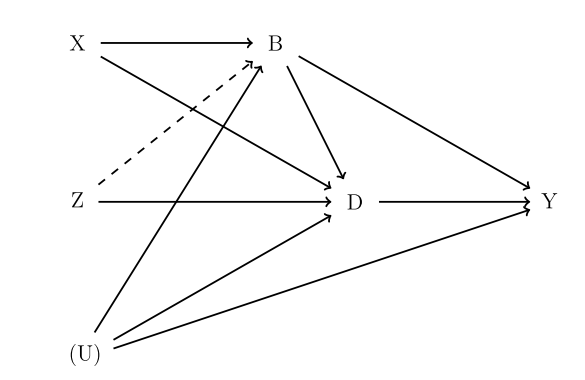
\includegraphics{figs/IE_diagrama.PNG}
\end{frame}

\begin{frame}{Posibles soluciones}
\protect\hypertarget{posibles-soluciones}{}
\begin{enumerate}
\item
  Estímulo abstracto
\item
  Control de covariables
\item
  Incorporar experimentos naturales
\end{enumerate}
\end{frame}

\begin{frame}{Limitaciones de los experimentos para la identificación
causal}
\protect\hypertarget{limitaciones-de-los-experimentos-para-la-identificaciuxf3n-causal}{}
\begin{itemize}
\tightlist
\item
  Críticas al contexto experimental
\item
  Críticas a los sujetos participantes de la encuesta
  (muestra)\footnote<.->{Coppock, Alexander. 2018. ``Generalizing from
    Survey Experiments Conducted on Mechanical Turk: A Replication
    Approach.'' Political Science Research and Methods. 1--16}
\end{itemize}
\end{frame}

\begin{frame}{Ventajas de los experimentos de encuesta}
\protect\hypertarget{ventajas-de-los-experimentos-de-encuesta}{}
\begin{itemize}
\tightlist
\item
  Son rentables
\item
  Pueden realizarse de forma rápida
\item
  Pueden incluirse en encuestas masivas en línea porque no requieren
  contacto en persona para su realización
\end{itemize}
\end{frame}

\hypertarget{experimentos-de-laboratorio}{%
\section{Experimentos de
Laboratorio}\label{experimentos-de-laboratorio}}

\begin{frame}{Lecturas}
\protect\hypertarget{lecturas-3}{}
\begin{itemize}
\tightlist
\item
  Falk \& Heckman, 2009: Las Experiments Are a Major Source of Knowledge
  in the Social Sciences
\item
  Habyarimana, et al., 2007: Why Do Ethnic Diversity Undermine Public
  Goods Provision?
\item
  Levine \& Palfrey, 2007: The Paradox of Voter Participation? A
  Laboratory Study
\item
  Levitt \& List, 2007: What Do Laboratory Experiments Measuring Social
  Preferences Reveal About the Real World?
\item
  Oxley, et al., 2008: Political Attitudes Vary with Physiological
  Traits
\end{itemize}
\end{frame}

\begin{frame}{Objetivos de los Experimentos}
\protect\hypertarget{objetivos-de-los-experimentos}{}
\begin{enumerate}
\item
  Testear teorías

  \begin{itemize}
  \tightlist
  \item
    Podemos implementar las condiciones de la teoría
  \item
    Comparar la predicción teórica con el resultado experimental
  \item
    Explorar las causas por las que una teoría falla
  \end{itemize}
\item
  Ofrecer modelos comportamentales

  \begin{itemize}
  \tightlist
  \item
    Estos describen el comportamiento en un contexto particular
  \end{itemize}
\item
  Establecer regularidades empíricas como base de nuevas teorías
\item
  Testear instituciones y ambientes
\item
  Evaluar propuestas de políticas
\item
  Revelación de las preferencias

  \begin{itemize}
  \tightlist
  \item
    Valoración
  \item
    Parámetros de la función de utilidad (tolerancia al riesgo,
    preferencia temporal, cooperación)
  \end{itemize}
\end{enumerate}
\end{frame}

\begin{frame}{Experimentos para medir preferencias sociales}
\protect\hypertarget{experimentos-para-medir-preferencias-sociales}{}
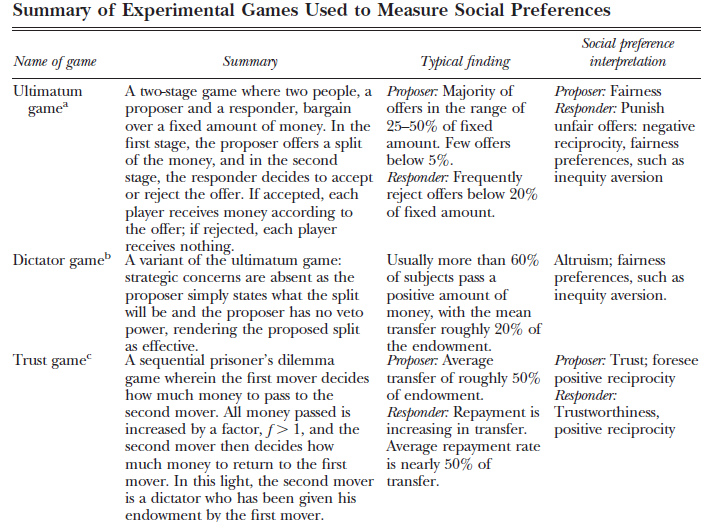
\includegraphics{figs/lab_social_preferences1.png}
\end{frame}

\begin{frame}{Experimentos para medir preferencias sociales}
\protect\hypertarget{experimentos-para-medir-preferencias-sociales-1}{}
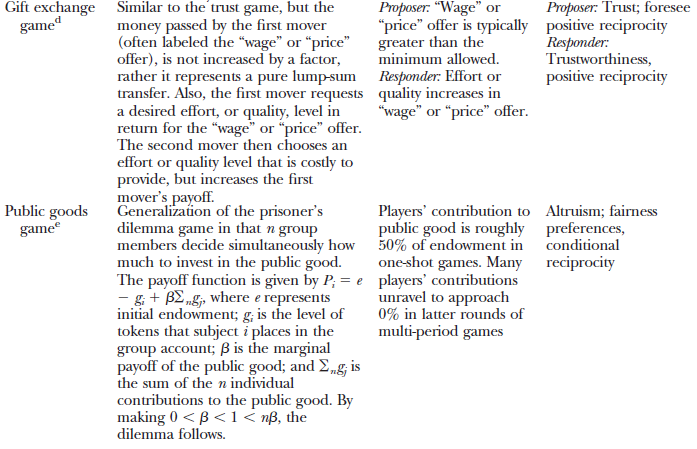
\includegraphics{figs/lab_social_preferences2.png}
\end{frame}

\begin{frame}{Ventajas de los experimentos de laboratorio}
\protect\hypertarget{ventajas-de-los-experimentos-de-laboratorio}{}
\begin{itemize}
\tightlist
\item
  Variación controlada:

  \begin{itemize}
  \tightlist
  \item
    Podemos mantener todo lo demás constante y cambiar de a una variable
    a la vez
  \item
    Permite un control estricto de los entornos de decisión, de las
    covariables
  \item
    Esto aplica, en particular, para testear modelos y supuestos
    comportamentales (teoría de juegos)
  \end{itemize}
\item
  Replicabilidad

  \begin{itemize}
  \tightlist
  \item
    Suele ser más difícil en los otros tipos de experimentos
  \end{itemize}
\end{itemize}
\end{frame}

\begin{frame}{Limitaciones de los experimentos de laboratorio}
\protect\hypertarget{limitaciones-de-los-experimentos-de-laboratorio}{}
\begin{enumerate}
\tightlist
\item
  \textit{Los experimentos no son realistas}

  \begin{itemize}
  \tightlist
  \item
    La simplicidad es una virtud: permite centrarse en los elementos
    clave
  \end{itemize}
\item
  \textit{Los experimentos son artificiales}

  \begin{itemize}
  \tightlist
  \item
    Grupo de sujetos sesgado (estudiantes)

    \begin{itemize}
    \tightlist
    \item
      Se puede utilizar otros sujetos
    \end{itemize}
  \item
    Número reducido de participantes

    \begin{itemize}
    \tightlist
    \item
      Se puede aumentar el número de participantes
    \end{itemize}
  \item
    Sujetos inexpertos

    \begin{itemize}
    \tightlist
    \item
      Se puede reclutar participantes con experiencia
    \end{itemize}
  \end{itemize}
\item
  \textit{Límites de los experimentos}

  \begin{itemize}
  \tightlist
  \item
    El control nunca es perfecto

    \begin{itemize}
    \tightlist
    \item
      El tiempo, el entorno del laboratorio condiciona el comportamiento
    \item
      No hay control real sobre los demás motivos
    \end{itemize}
  \end{itemize}
\item
  Los problemas de siempre (también los tienen otros tipos de
  experimentos):

  \begin{itemize}
  \tightlist
  \item
    Autoselección de los participantes
  \item
    Validez externa
  \end{itemize}
\end{enumerate}
\end{frame}

\begin{frame}{¿Qué hay que diseñar?}
\protect\hypertarget{quuxe9-hay-que-diseuxf1ar}{}
\begin{itemize}
\tightlist
\item
  Pensar sobre los datos necesarios para responder la pregunta

  \begin{itemize}
  \tightlist
  \item
    Recolectar todo lo relevante
  \item
    Obtener información sobre confounders siempre que se pueda
  \item
    Asegurarse que la cantidad de jugadores sea suficiente para
    encontrar significancia (a través de simulaciones, por ej.)
  \end{itemize}
\item
  Intentar que las instrucciones sean claras y el juego simple

  \begin{itemize}
  \tightlist
  \item
    Se puede realizar un pre-test (piloto)
  \end{itemize}
\end{itemize}
\end{frame}

\begin{frame}{¿Qué hay que diseñar?}
\protect\hypertarget{quuxe9-hay-que-diseuxf1ar-1}{}
Hay que pensar varias cosas a la hora de diseñar un experimento de
laboratorio

\begin{itemize}
\tightlist
\item
  El ambiente:

  \begin{itemize}
  \tightlist
  \item
    Agentes (cantidad, tipo -estudiantes o no-, motivación)
  \item
    Materias primas: ¿Sobre qué se toman las decisiones?
  \item
    Dotaciones: ¿De qué disponen al iniciar el experimento los tomadores
    de decisiones?
  \item
    Mecanismo por el que puede producirse el aprendizaje (oportunidades
    de búsqueda, práctica)
  \end{itemize}
\item
  Institución:

  \begin{itemize}
  \tightlist
  \item
    Decisiones a disposición de los sujetos

    \begin{itemize}
    \tightlist
    \item
      Reglas sobre las decisiones
    \item
      Reglas sobre la comunicación
    \end{itemize}
  \item
    Conexión entre decisiones y retribuciones
  \end{itemize}
\end{itemize}
\end{frame}

\begin{frame}{¿Reclutar estudiantes o poblacipon general?}
\protect\hypertarget{reclutar-estudiantes-o-poblacipon-general}{}
Estudiantes:

\begin{itemize}
\item
  Normalmente más fáciles de reclutar
\item
  Se pueden conducir experimentos más difíciles
\item
  Aprenden más rápido
\item
  Tienen limitada experiencia de la ``vida real'', pero no confundirán
  con ``vida real''
\item
  Evitar estudiantes de misma clase o grupo (salvo que sea el objetivo
  del estudio)
\end{itemize}
\end{frame}

\begin{frame}{¿Participantes conocidos o extraños?}
\protect\hypertarget{participantes-conocidos-o-extrauxf1os}{}
\begin{itemize}
\tightlist
\item
  Conocidos:

  \begin{itemize}
  \tightlist
  \item
    El grupo está formado por los mismos sujetos
  \item
    Comportamiento estratégico
  \end{itemize}
\item
  Extraños:

  \begin{itemize}
  \tightlist
  \item
    En cada período se creará un nuevo grupo con nuevos sujetos
  \end{itemize}
\item
  Extraños perfectos:

  \begin{itemize}
  \tightlist
  \item
    Los sujetos nunca se encontrarán con los mismos sujetos en el futuro
  \end{itemize}
\end{itemize}
\end{frame}

\begin{frame}{¿Cuántos?}
\protect\hypertarget{cuuxe1ntos}{}
\begin{itemize}
\item
  Depende del tipo de experimento
\item
  Regla general: no menos que los experimentos previos en el área
\item
  Asegurarse que hay suficientes participantes para cada sesión:

  \begin{itemize}
  \tightlist
  \item
    Reclutar algunos más de los necesarios
  \item
    Esto es más importante aún cuando los participantes interactúan
  \end{itemize}
\item
  \textbf{Algunas reglas sobre el reclutamiento}

  \begin{itemize}
  \tightlist
  \item
    No promesas falsas
  \item
    No decirles cuánto dinero ganarán, pero sí decirles que van a ganar
    algo de dinero incluyendo un pago por presentarse
  \item
    Decirles que es un experimento que estudia comportamiento humano o
    toma de decisiones
  \end{itemize}
\end{itemize}
\end{frame}

\begin{frame}{¿Un período o varios períodos?}
\protect\hypertarget{un-peruxedodo-o-varios-peruxedodos}{}
Un periodo

\begin{itemize}
\tightlist
\item
  No hay incentivos estratégicos
\item
  No hay derrames entre períodos
\item
  Fácil y rápido de conducir
\end{itemize}

Multi-periodos

\begin{itemize}
\tightlist
\item
  Hay incentivos estratégicos
\item
  Efectos dinámicos

  \begin{itemize}
  \tightlist
  \item
    Por ejemplo: convergencia hacia 0 contribución en juego de bienes
    públicos
  \end{itemize}
\item
  Efectos de aprendizaje
\item
  Más observaciones
\end{itemize}
\end{frame}

\begin{frame}{Recompensas}
\protect\hypertarget{recompensas}{}
\begin{itemize}
\item
  Pueden ser en:

  \begin{itemize}
  \tightlist
  \item
    Efectivo
  \item
    Tasa de cambio fijo entre las unidades monetarias experimentales y
    la moneda local
  \end{itemize}
\item
  A menos que el tamaño de la apuesta sea la cuestión de la
  investigación, se debe calibrar con una ganancia media en torno al
  coste de oportunidad de lo sujetos
\item
  Si es posible que se produzcan pérdidas en los experimentos, esto debe
  indicarse claramente, incluyendo cómo cubrir las pérdidas (por
  ejemplo, con el pago por participación) y si los sujetos pueden dejar
  de participar en el experimento en caso de sufrir pérdidas
\end{itemize}
\end{frame}

\begin{frame}{Condiciones para los incentivos}
\protect\hypertarget{condiciones-para-los-incentivos}{}
\begin{itemize}
\item
  Los sujetos deben preferir obtener más recompensa, y no saciarse
\item
  La recompensa depende de las acciones del sujeto (sin contar el pago
  por participación)
\item
  Los cambios en la utilidad de un sujeto a partir del experimento
  provienen predominantemente de la recompensa, y la influencia de los
  otros motivos es insignificante (este supuesto es el más crítico)
\item
  Si se cumplen estas condiciones, el experimentador controla las
  preferencias de los sujetos
\end{itemize}
\end{frame}

\begin{frame}{A tener en cuenta:}
\protect\hypertarget{a-tener-en-cuenta}{}
\begin{itemize}
\tightlist
\item
  Los beneficios para los demás pueden ser importantes para un
  participante

  \begin{itemize}
  \tightlist
  \item
    Envidia
  \item
    Equidad
  \end{itemize}
\item
  Deseo de complacer al experimentador

  \begin{itemize}
  \tightlist
  \item
    Hace que las personas tomen acciones que no tomarían en al vida real
  \end{itemize}
\item
  Posibles soluciones

  \begin{itemize}
  \tightlist
  \item
    Hacer que el cambio en los beneficios monetarios sea lo
    suficientemente grande
  \item
    Evitar la información pública sobre los beneficios
  \item
    No dar pistas sobre el objetivo del experimento
  \item
    Utilizar un lenguaje neutro en las instrucciones
  \end{itemize}
\end{itemize}
\end{frame}

\begin{frame}{Rondas de práctica}
\protect\hypertarget{rondas-de-pruxe1ctica}{}
\begin{itemize}
\item
  Sirven para incrementar el entendimiento del experimento
\item
  Pero puede afectar el comportamiento futuro

  \begin{itemize}
  \tightlist
  \item
    Las personas pueden inferir a partir del comportamiento en las
    rondas de práctica
  \end{itemize}
\item
  Pérdida de información sobre las acciones en el primer período
\end{itemize}
\end{frame}

\begin{frame}{Cuestionarios}
\protect\hypertarget{cuestionarios}{}
\begin{itemize}
\item
  Preguntas socio-económicas
\item
  Preguntas sobre los motivos del comportamiento en el experimento
\item
  Preguntas sobre comprensión del experimento
\end{itemize}
\end{frame}

\begin{frame}{¿Experimento en papel o informatizado?}
\protect\hypertarget{experimento-en-papel-o-informatizado}{}
Los experimentos informatizados tienen las siguientes ventajas:

\begin{itemize}
\item
  Son más simples y rápidos de correr
\item
  Menos errores
\item
  Menos interacción con el experimentalista
\item
  Los datos se recogen automáticamente
\item
  Interacción en directo
\item
  Interfaces dinámicas
\end{itemize}

Pero:

\begin{itemize}
\item
  No es visible
\item
  Lleva tiempo la programación
\item
  No es posible en todas las circunstancias
\end{itemize}
\end{frame}

\begin{frame}{Programas informáticos especializados}
\protect\hypertarget{programas-informuxe1ticos-especializados}{}
\begin{itemize}
\tightlist
\item
  z-Tree (Fischbacher, 2007)

  \begin{itemize}
  \tightlist
  \item
    Zurich Toolbox for Readymade Economic Experiments -
    \url{http://www.iew.unizh.ch/ztree/index.php}
  \item
    Se ejecuta localmente
  \end{itemize}
\item
  oTree (Chen, Schonger y Wickens, 2016)

  \begin{itemize}
  \tightlist
  \item
    Es un software emergente
  \item
    Independiente de la plataforma, basado en la web
  \end{itemize}
\end{itemize}
\end{frame}

\end{document}
